%=== Préambule ===========================================================

\documentclass{beamer}
\usepackage{pdfpages}
\usepackage[english]{babel}
\usepackage{xspace}
\usepackage{pifont}
\usepackage{hyperref}
\usepackage{listings}
\usepackage{csquotes}
\usepackage{graphicx}
\usepackage{animate,media9} %,movie15}
\usepackage{wrapfig}
\usepackage{pdfpages}
\usepackage{tikz}
\usepackage{natbib}
\uselanguage{English}
\usepackage{fontawesome5}
\languagepath{English}
\setcounter{tocdepth}{1}
\usepackage{setspace}
\usepackage{amsmath}
\def\glasses{{\sffamily 
\leavevmode\rlap{%
\rotatebox[origin=tr]{125}{J}\kern1ex%  
\rotatebox[origin=tr]{125}{J}}% 
\rotatebox[origin=c]{-90}{D}%   
\rotatebox[origin=c]{-90}{D}}%
\def\ialy{\sffamily 
\resizebox{1ex}{1.5ex}{\reflectbox{\rotatebox[origin=]{75}{J}}}\kern-1pt%
\rlap{\tiny$\ ^\bullet\kern2.5pt^\bullet$ }%
\rotatebox[origin=c]{-90}{D}%   
\rotatebox[origin=c]{-90}{D}\kern-1pt%  
\resizebox{1ex}{1.5ex}{\rotatebox[origin=]{75}{J}}}}


\lstset{
  numbers=left,
  basicstyle=\tiny\ttfamily,      
  breaklines=true, 
  showtabs=false,
  showstringspaces=false,
}  

%=== Configuration de Beamer et du thème metropolis ======================
\usepackage{bbding}
\usetheme[background=light]{metropolis}
\usepackage[clock]{ifsym}

\definecolor{mLightBrown}{HTML}{000000}
\definecolor{black}{HTML}{000000}
\setbeamercolor{structure}{fg=black,bg=mLightBrown}
\setbeamercolor{palette primary}{%
	use=normal text,
	fg=normal text.bg,
	bg=mLightBrown
}
%\setsansfont[BoldFont={Linux Libertine G Bold},Numbers={OldStyle}]{Linux Libertine G}

\metroset{block=fill}

%=== Page de titre =======================================================

%path to logo and biblio -> to be adapted to your local directories 
\newcommand\dirlogo{../../logos/}
\newcommand\dirbiblio{../../biblio/}



\title{{\normalsize \vskip 1cm Exploring complex normal faulting systems through physics-based dynamic rupture modeling}}
\subtitle{\small 10-12 min talk!}
\author{Hugo S. \\ {\tiny Institut de Recherche pour le Développement IRD - ISTerre} \\ 
O., Scotti, S., Hok, A.-A. Gabriel and T. Taufiqurrahman \\
\\
\textit{ANR EQTIME Project}
}

\date[2021]{\today}

\subject{Group Meeting}

\titlegraphic{\centering \vspace{-15pt}
\includegraphics[height=1.3cm]{../../logos/logo_all_presentation.pdf} \par} %\qquad  
\includegraphics[height=1.4cm]{../../logos/anr_eqtime.png} \par }


\addtobeamertemplate{frametitle}{}{%
\begin{tikzpicture}[remember picture,overlay]
  \node[anchor=north east,yshift=0.0ex] at (current page.north east) {
\includegraphics[height=4ex]{../../logos/logo_irsn_neg}};
  %\node[anchor=north east,yshift=0.5ex] at (current page.north east) {\includegraphics[height=3.3ex]{\dirlogo/seiscope_color_light_background}};
\end{tikzpicture}}



%=== Document ============================================================

\begin{document}

% --- Préambule ---------------------------------------------------------------

\begin{frame}
    \titlepage
\end{frame}

\begin{frame}
 {Outline}
 
 \tableofcontents
 
\end{frame}



\section{Motivation}


\begin{frame}
 {Seismic Hazard in Central Italy}
 
 \begin{center}
 \begin{minipage}{0.65\linewidth}
  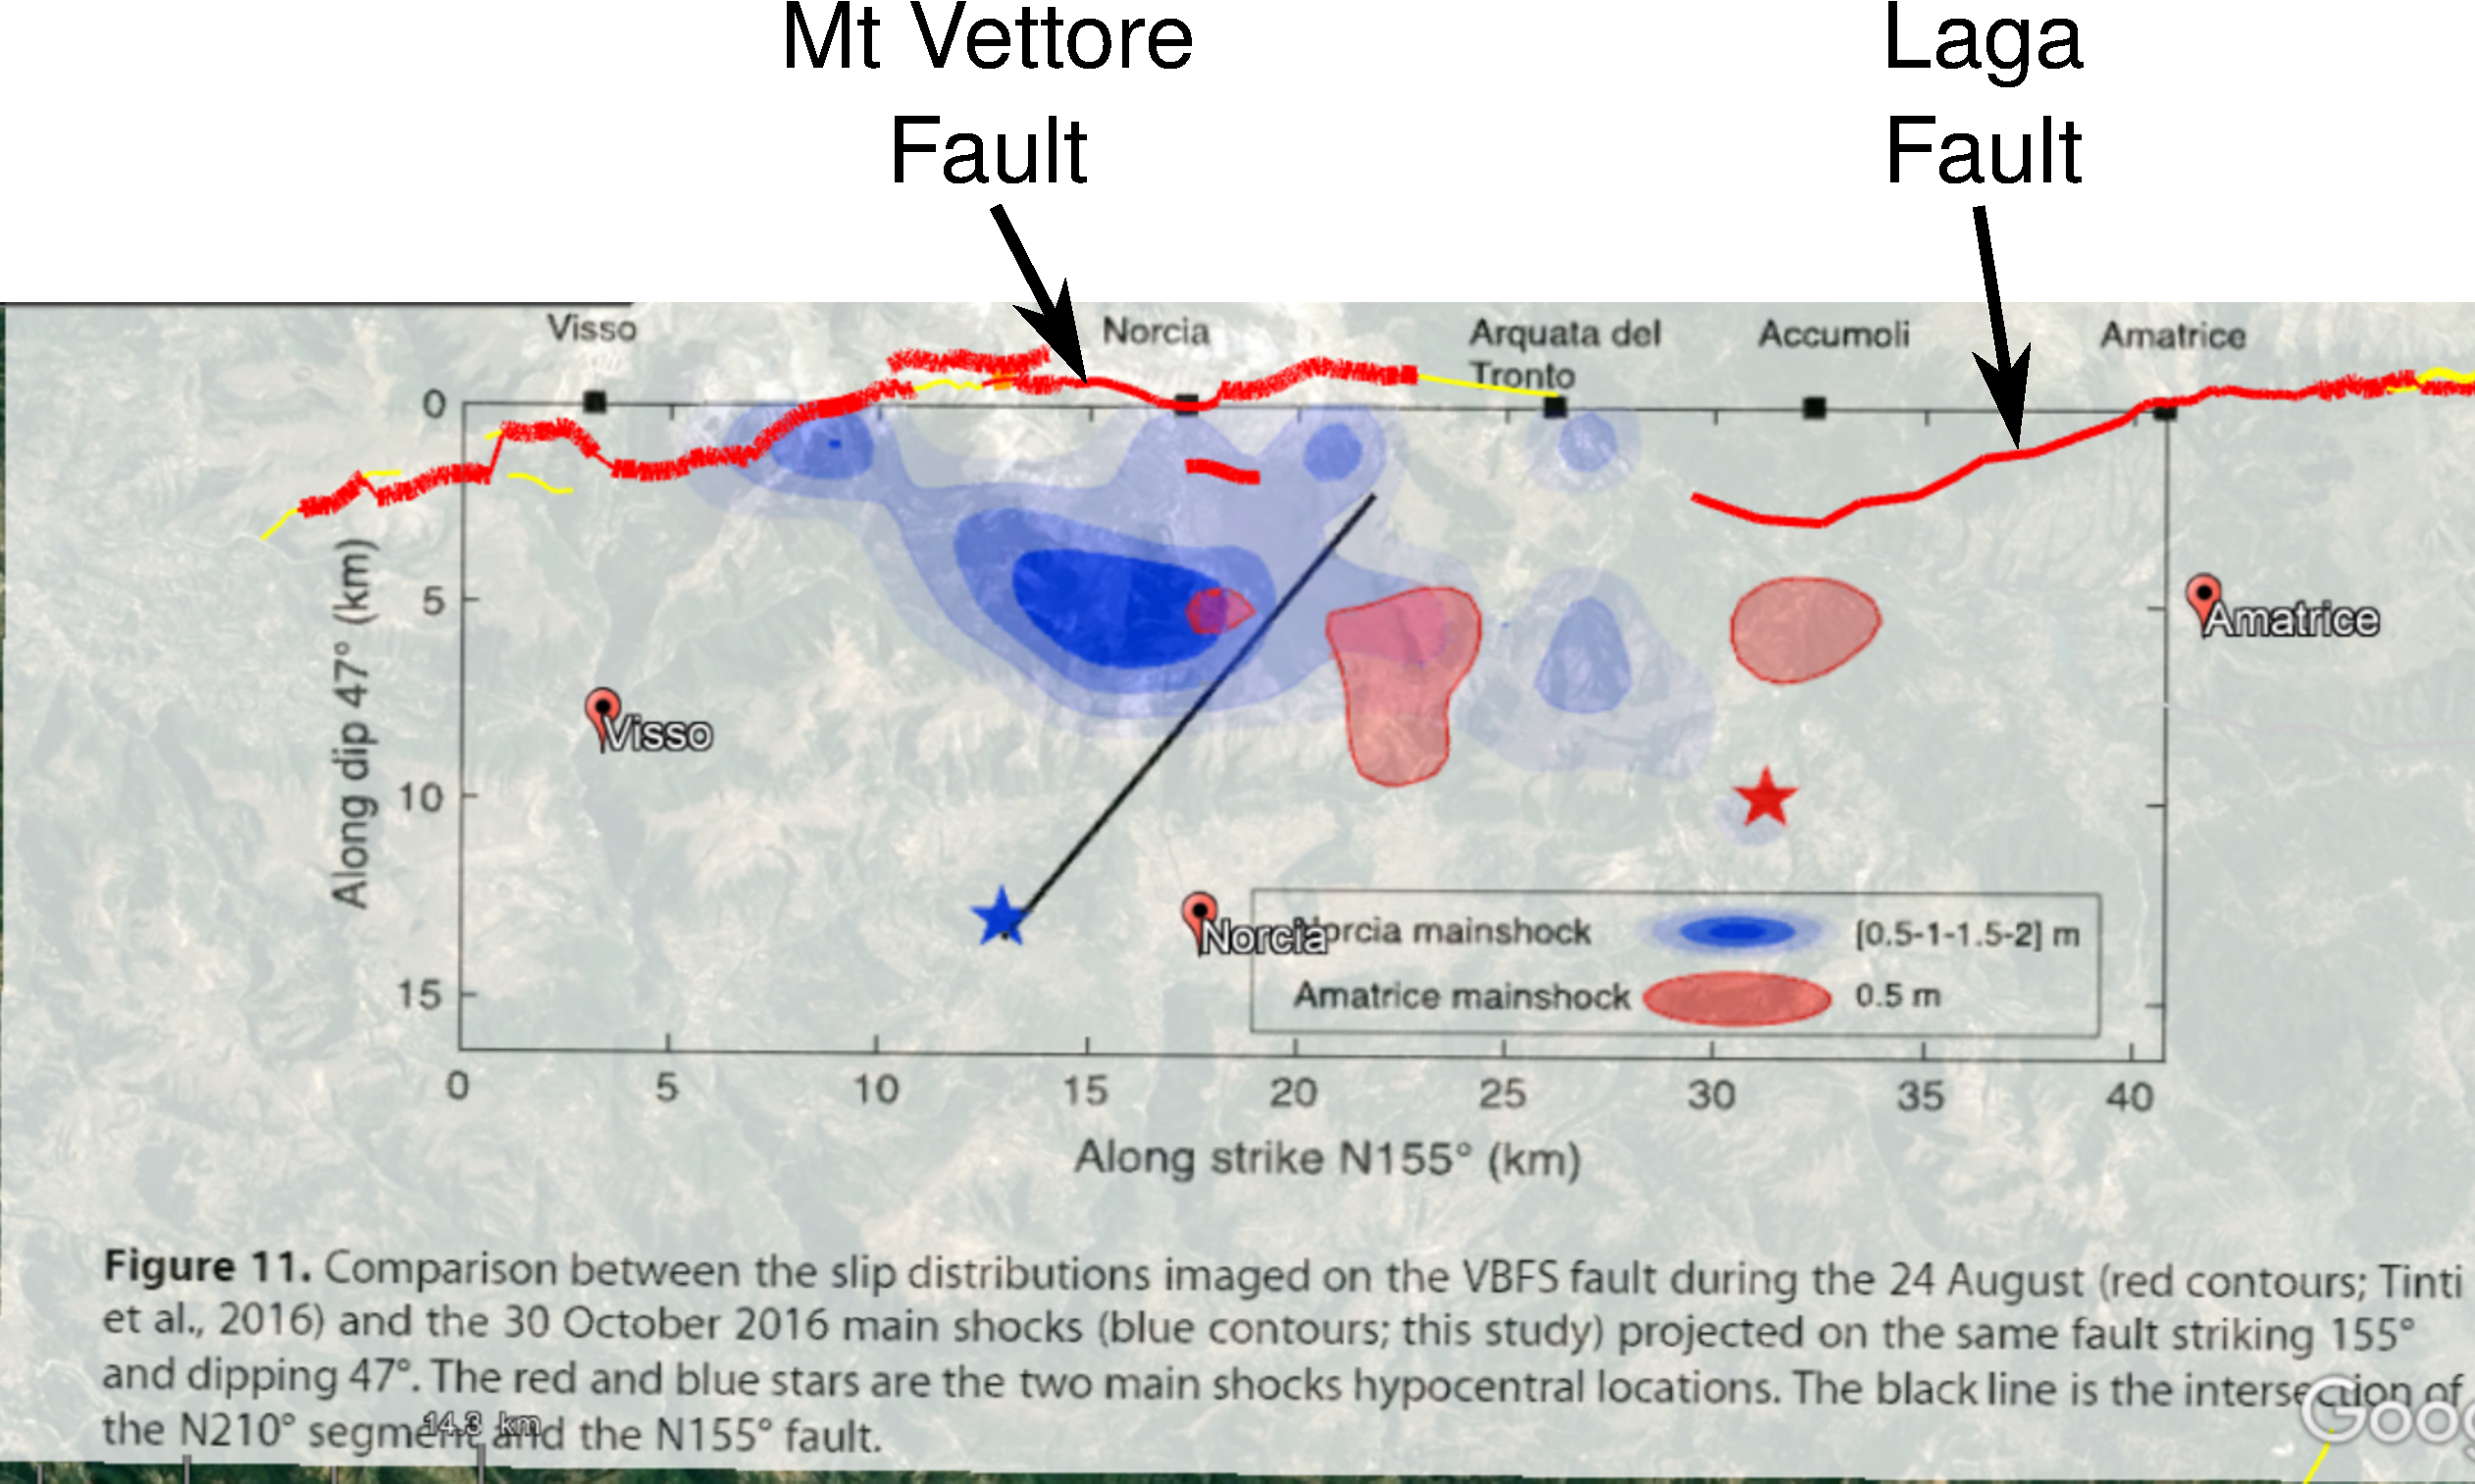
\includegraphics[width=1\linewidth]{images/amatrice_1.pdf} \,
  \vskip 0.2cm
  {\bf \tiny Modified by O. Scotti from \cite{Scognamiglio_2018_CFG}} \end{minipage}
 \begin{minipage}{0.33\linewidth}
  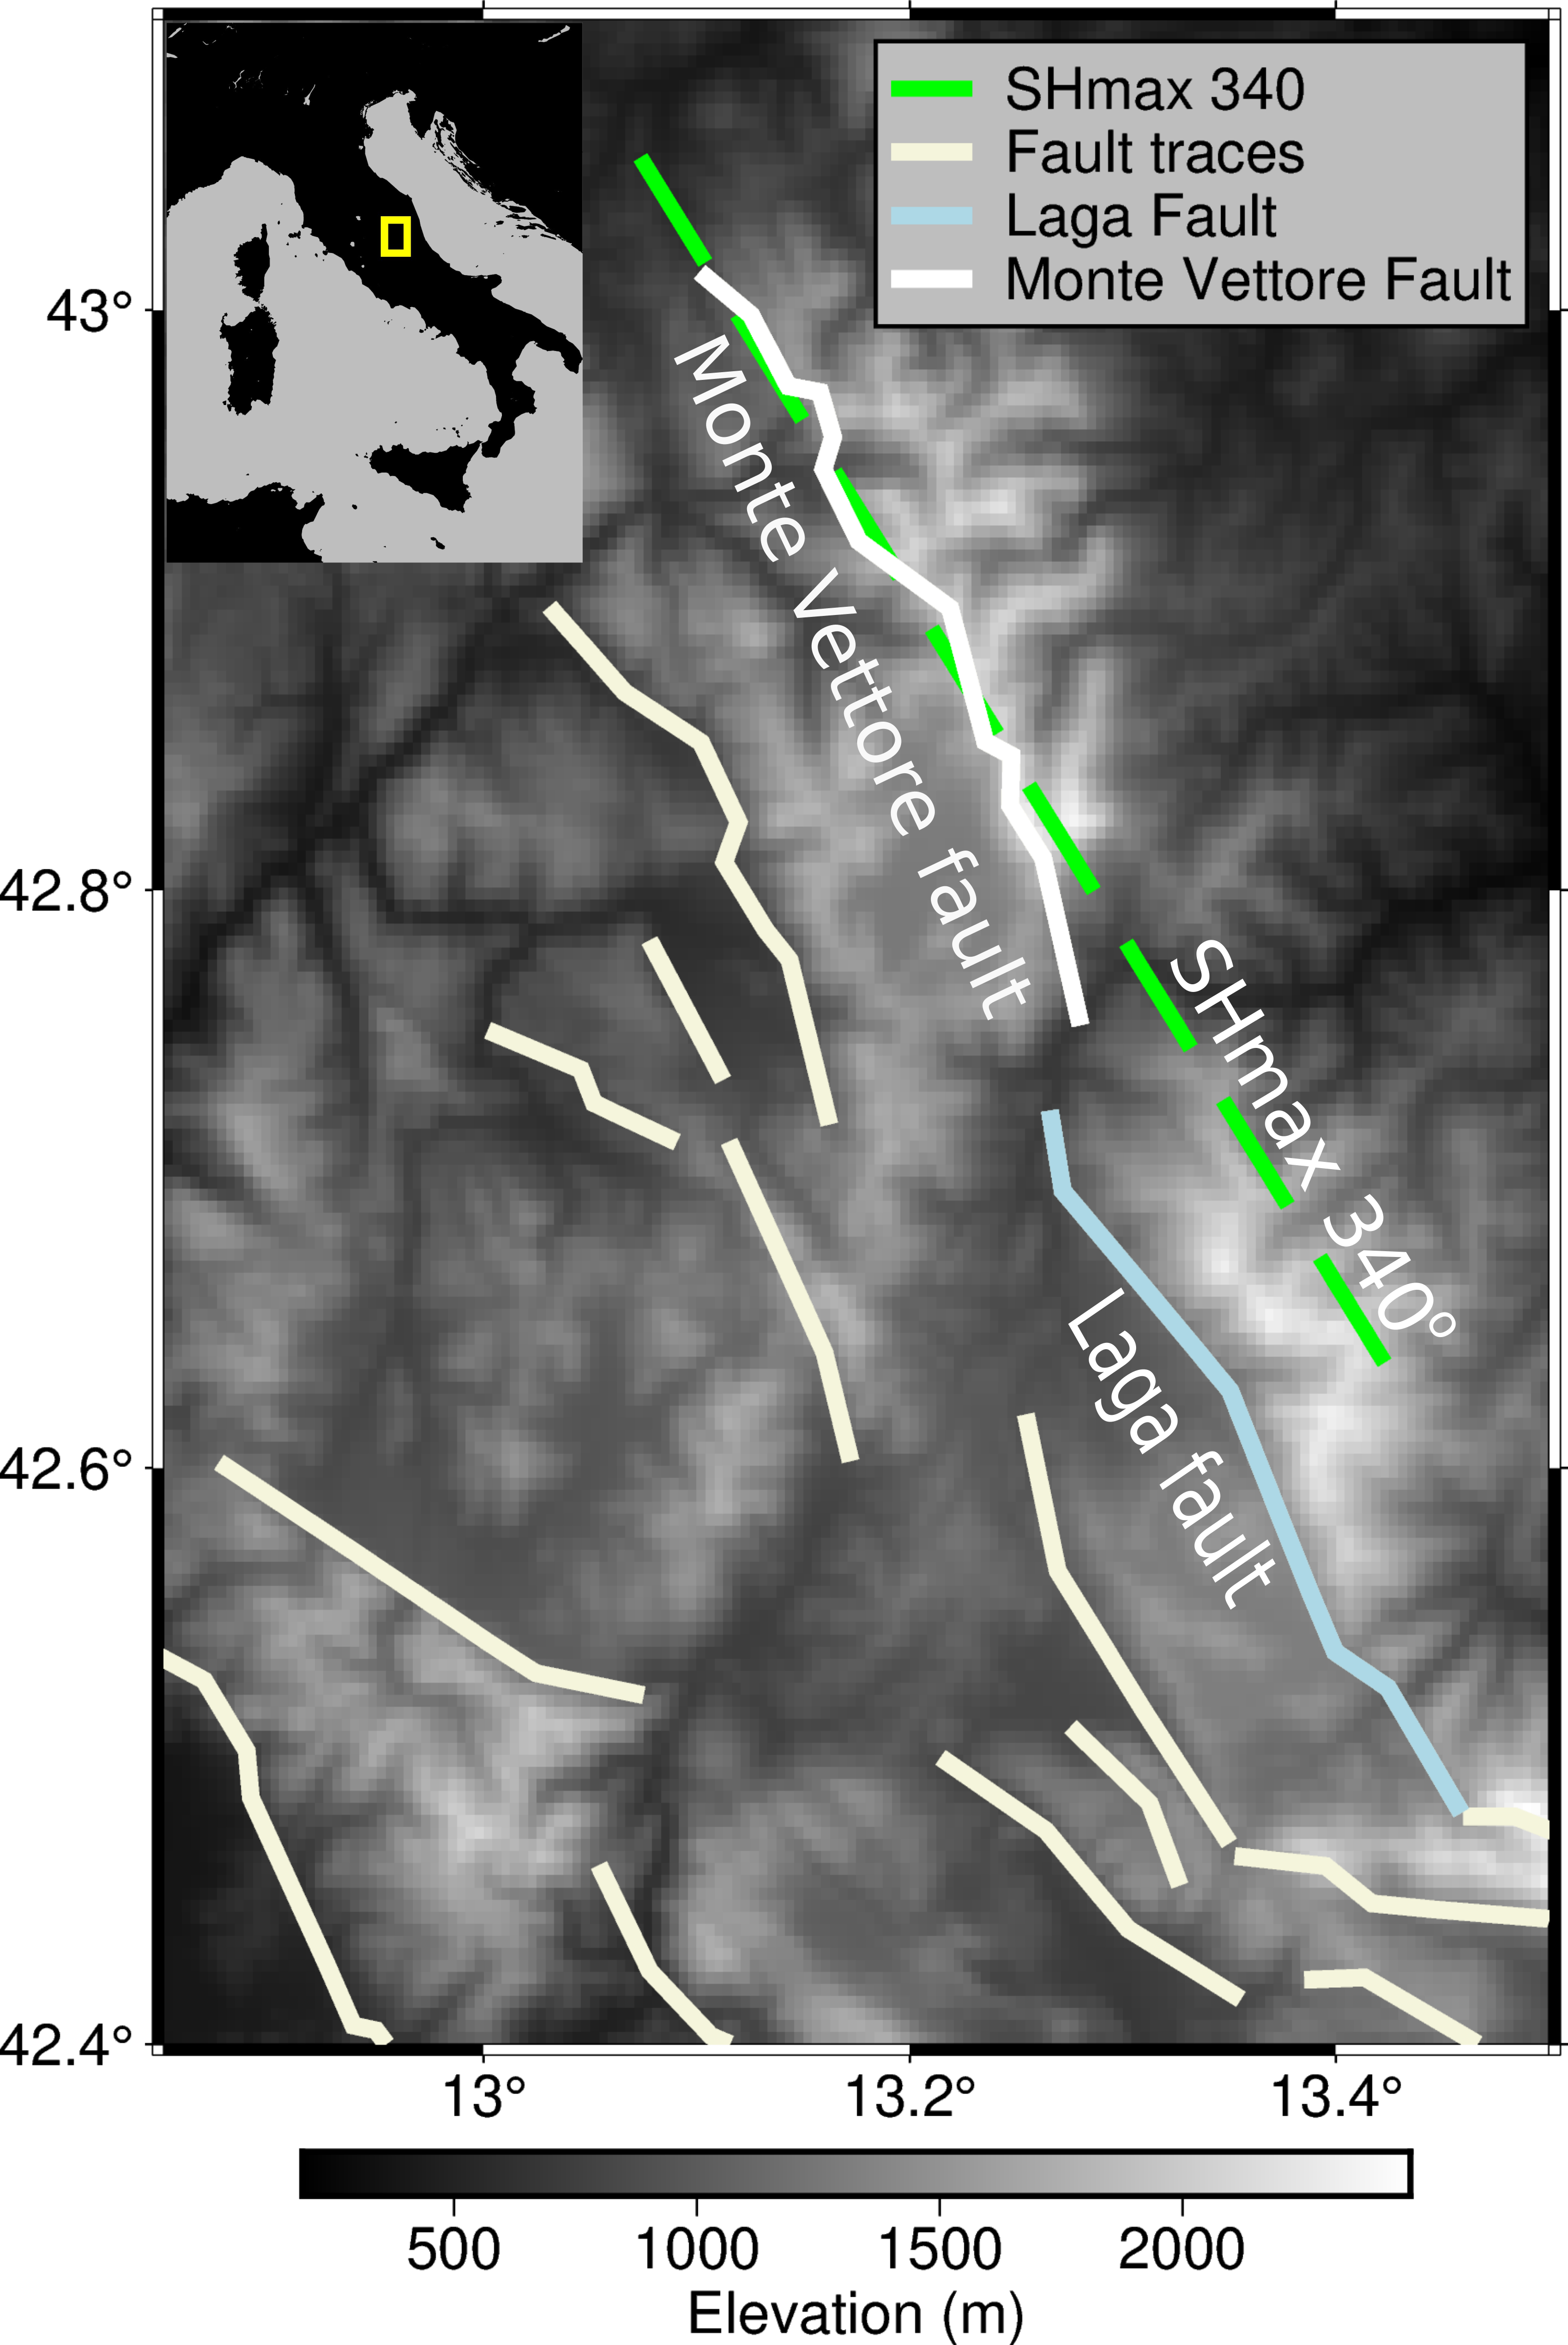
\includegraphics[width=1\linewidth]{images/Map_Italy.png}  
  \vskip 0.2cm
  {\bf \tiny Map based on \cite{Walker_2021_FAULT2SHA}} \end{minipage}
 \end{center}

  
\end{frame}

\begin{frame}
 {Seismic Hazard in Central Italy}
 
 \begin{center}
 \begin{center}
 \begin{minipage}{0.65\linewidth}
  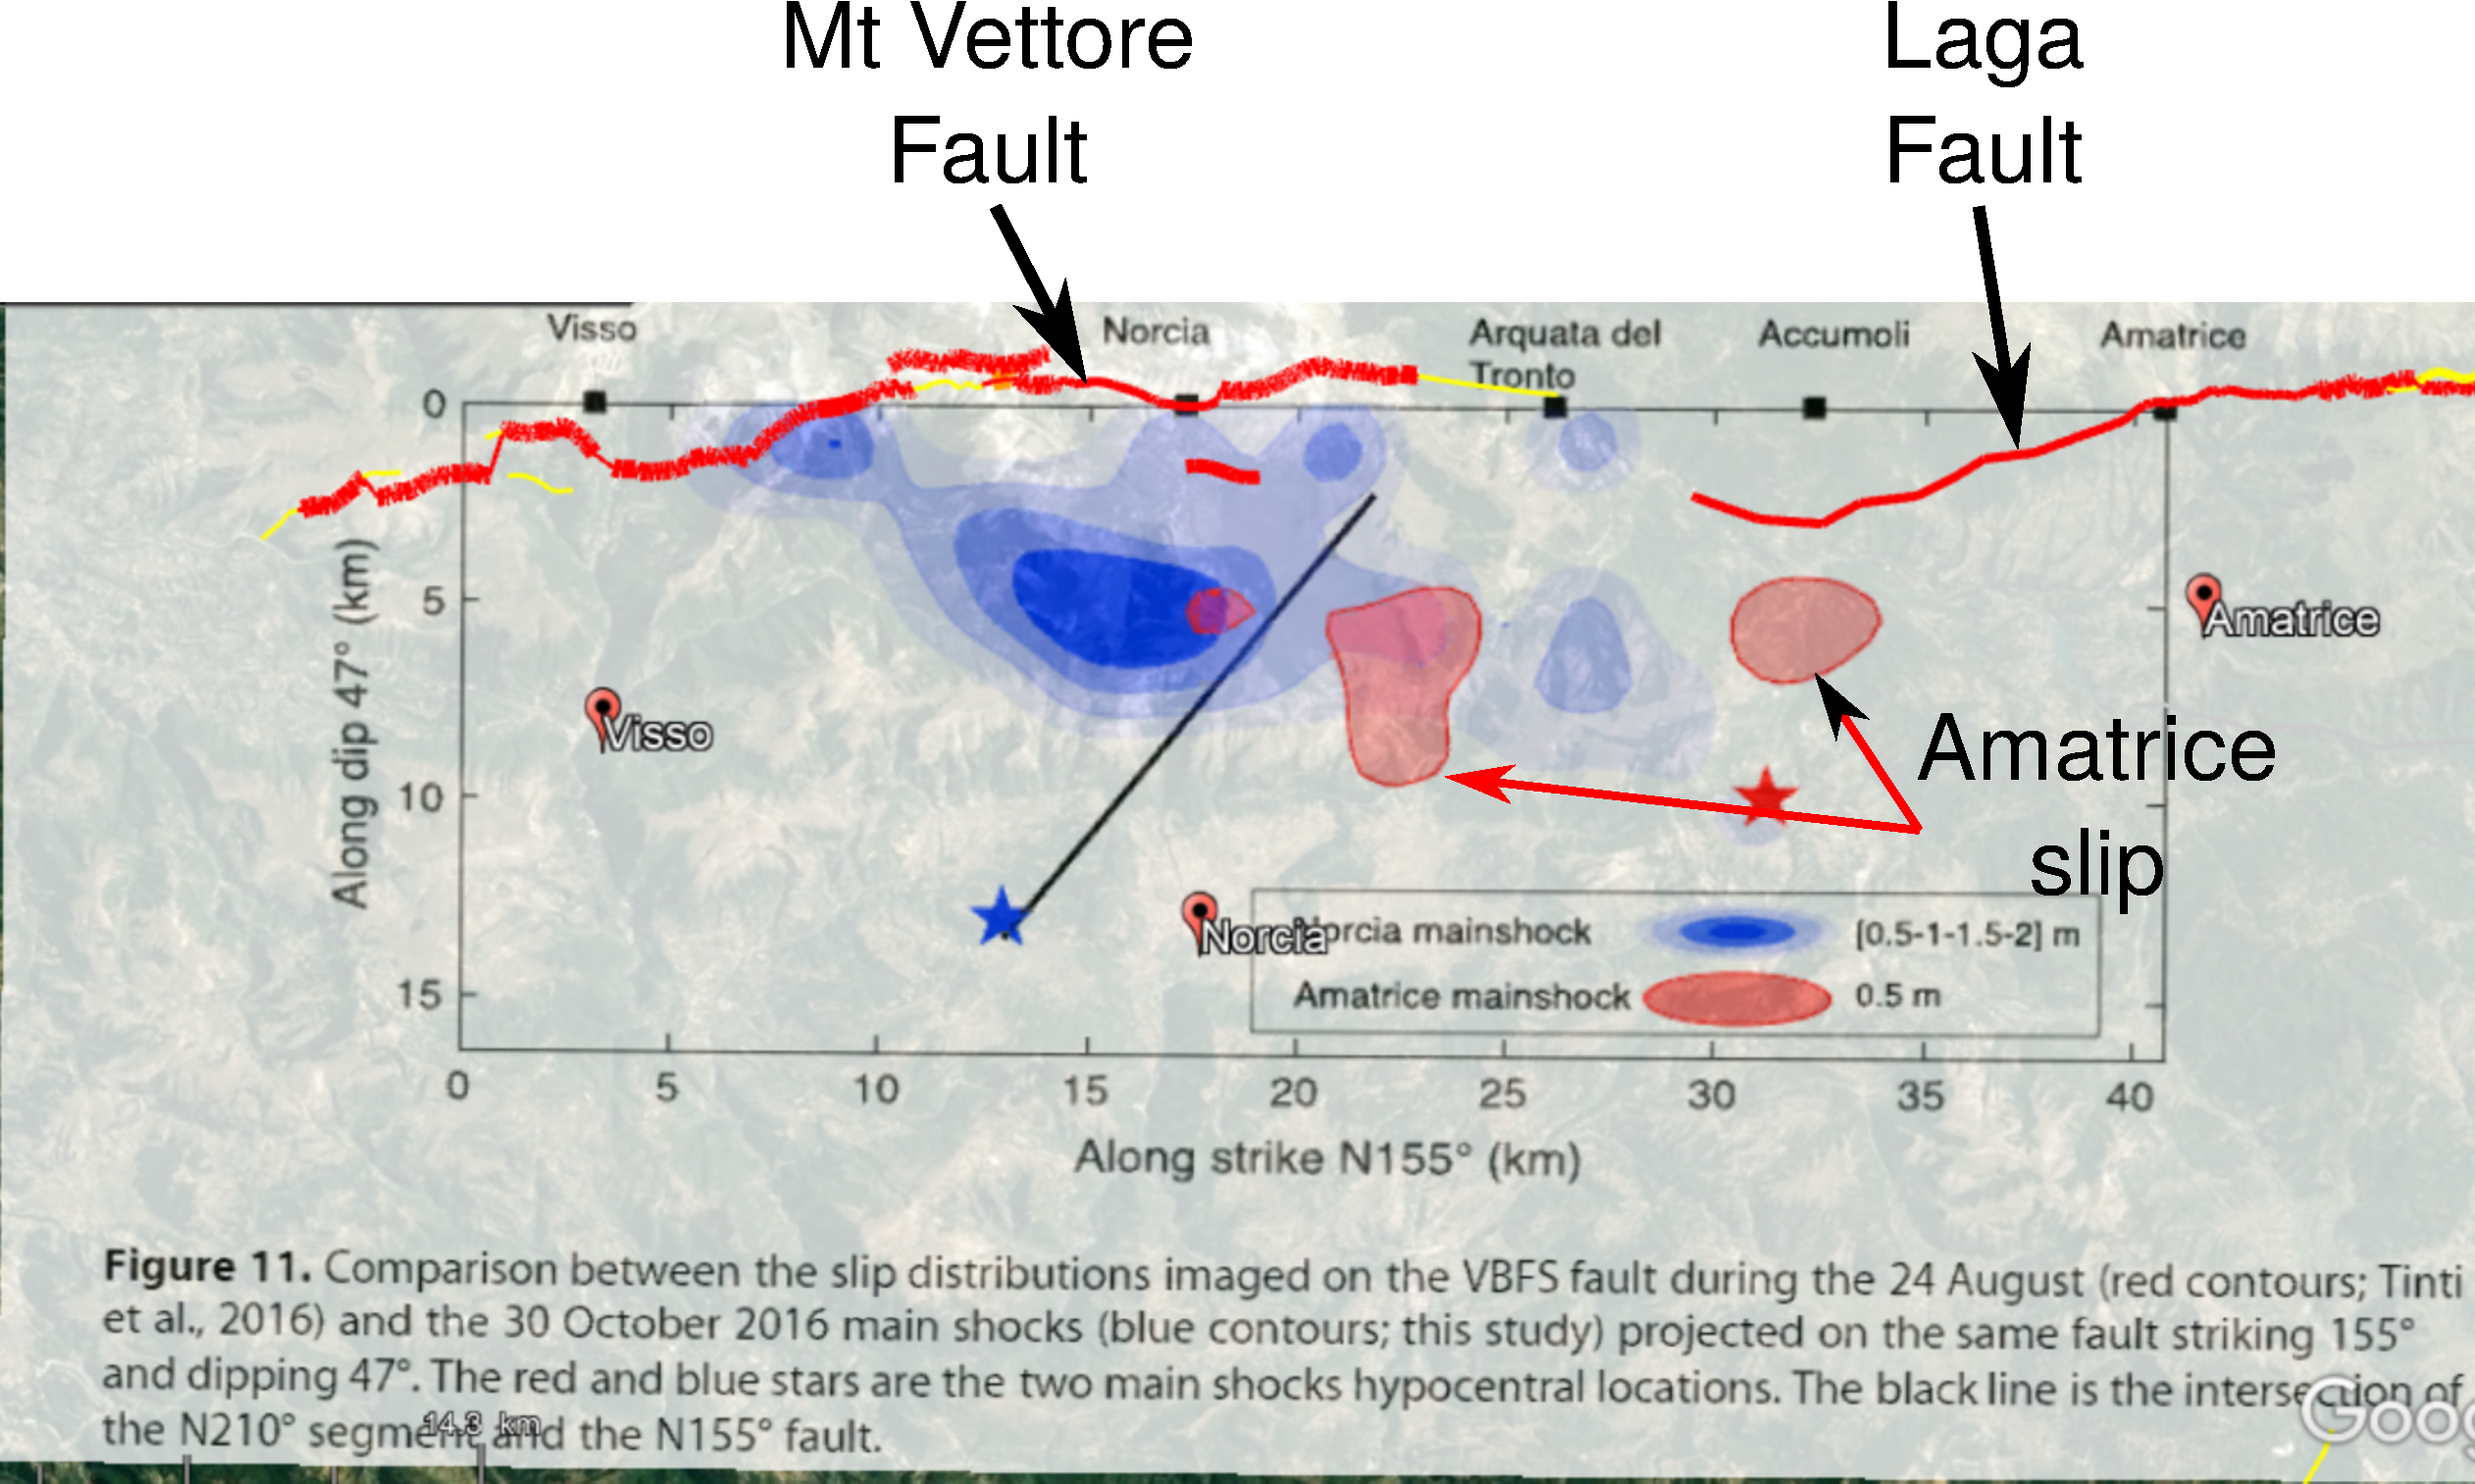
\includegraphics[width=1\linewidth]{images/amatrice_2.pdf} \,
  \vskip 0.2cm
  {\bf \tiny Modified by O. Scotti from \cite{Scognamiglio_2018_CFG}} \end{minipage}
 \begin{minipage}{0.33\linewidth}
  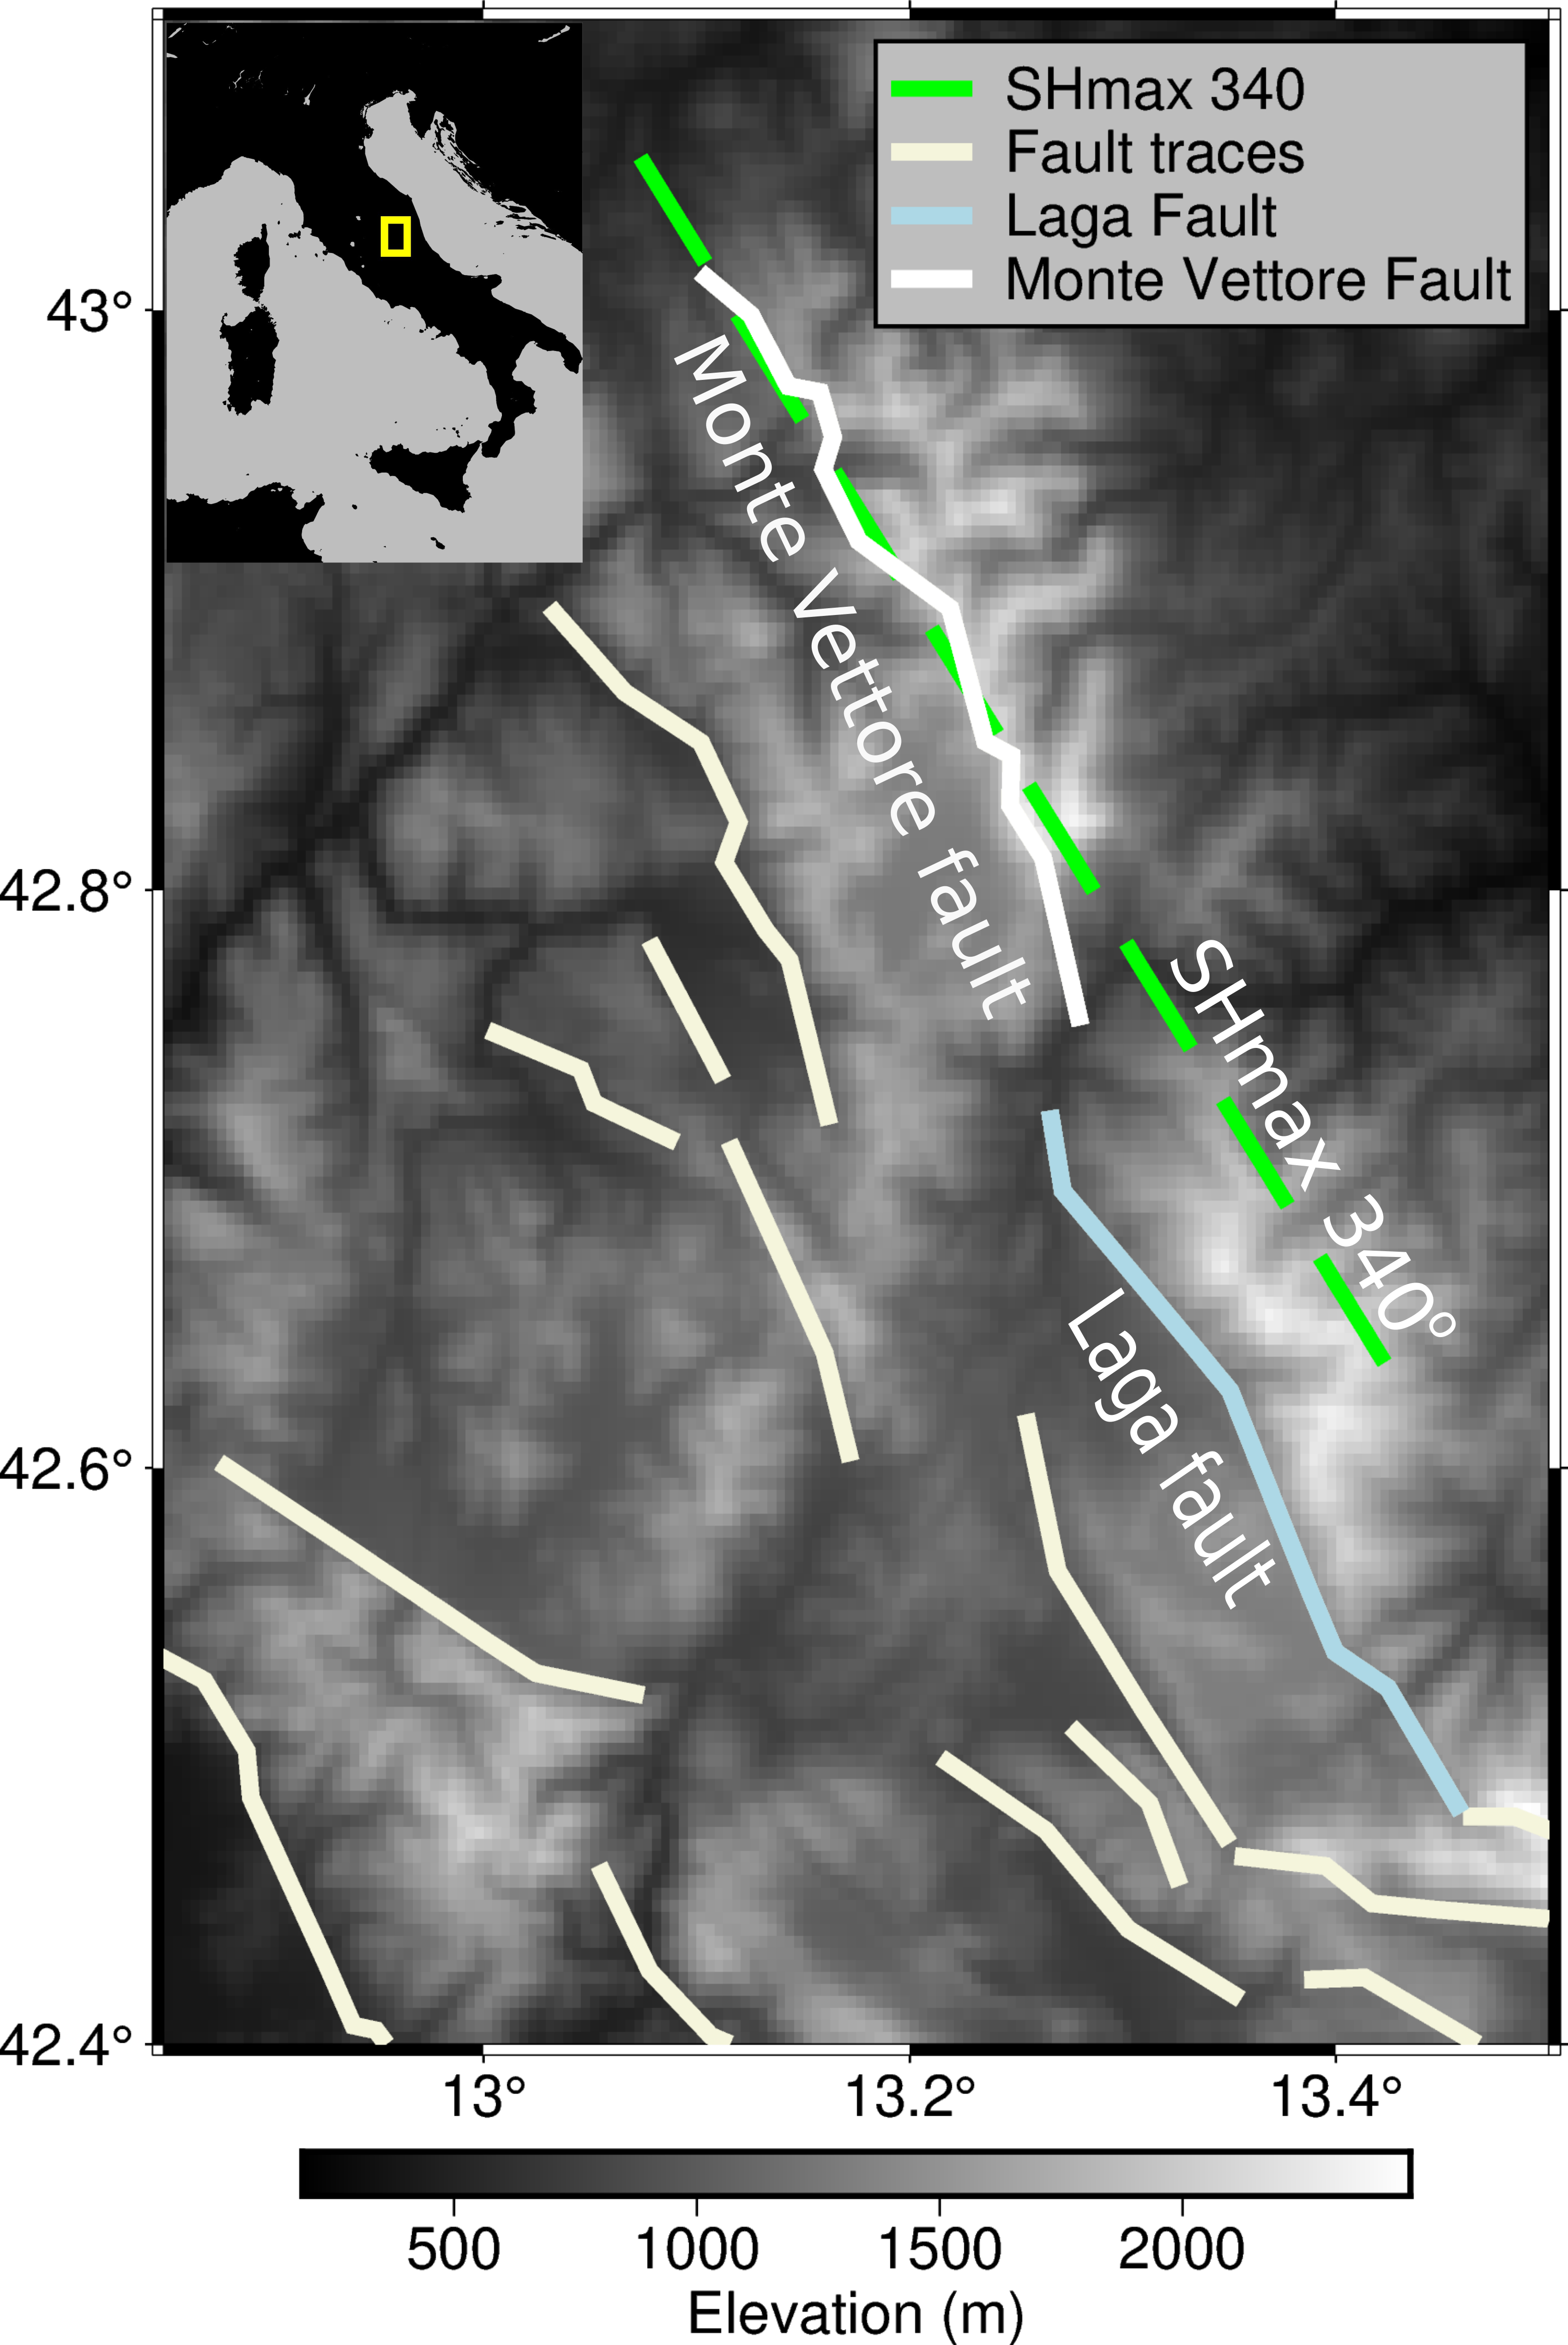
\includegraphics[width=1\linewidth]{images/Map_Italy.png}  
  \vskip 0.2cm
  {\bf \tiny Map based on \cite{Walker_2021_FAULT2SHA}} \end{minipage}
 \end{center}
 \end{center}
  \addtocounter{framenumber}{-1}
  
\end{frame}


\begin{frame}
 {Seismic Hazard in Central Italy}

 \begin{center}
 \begin{center}
 \begin{minipage}{0.65\linewidth}
  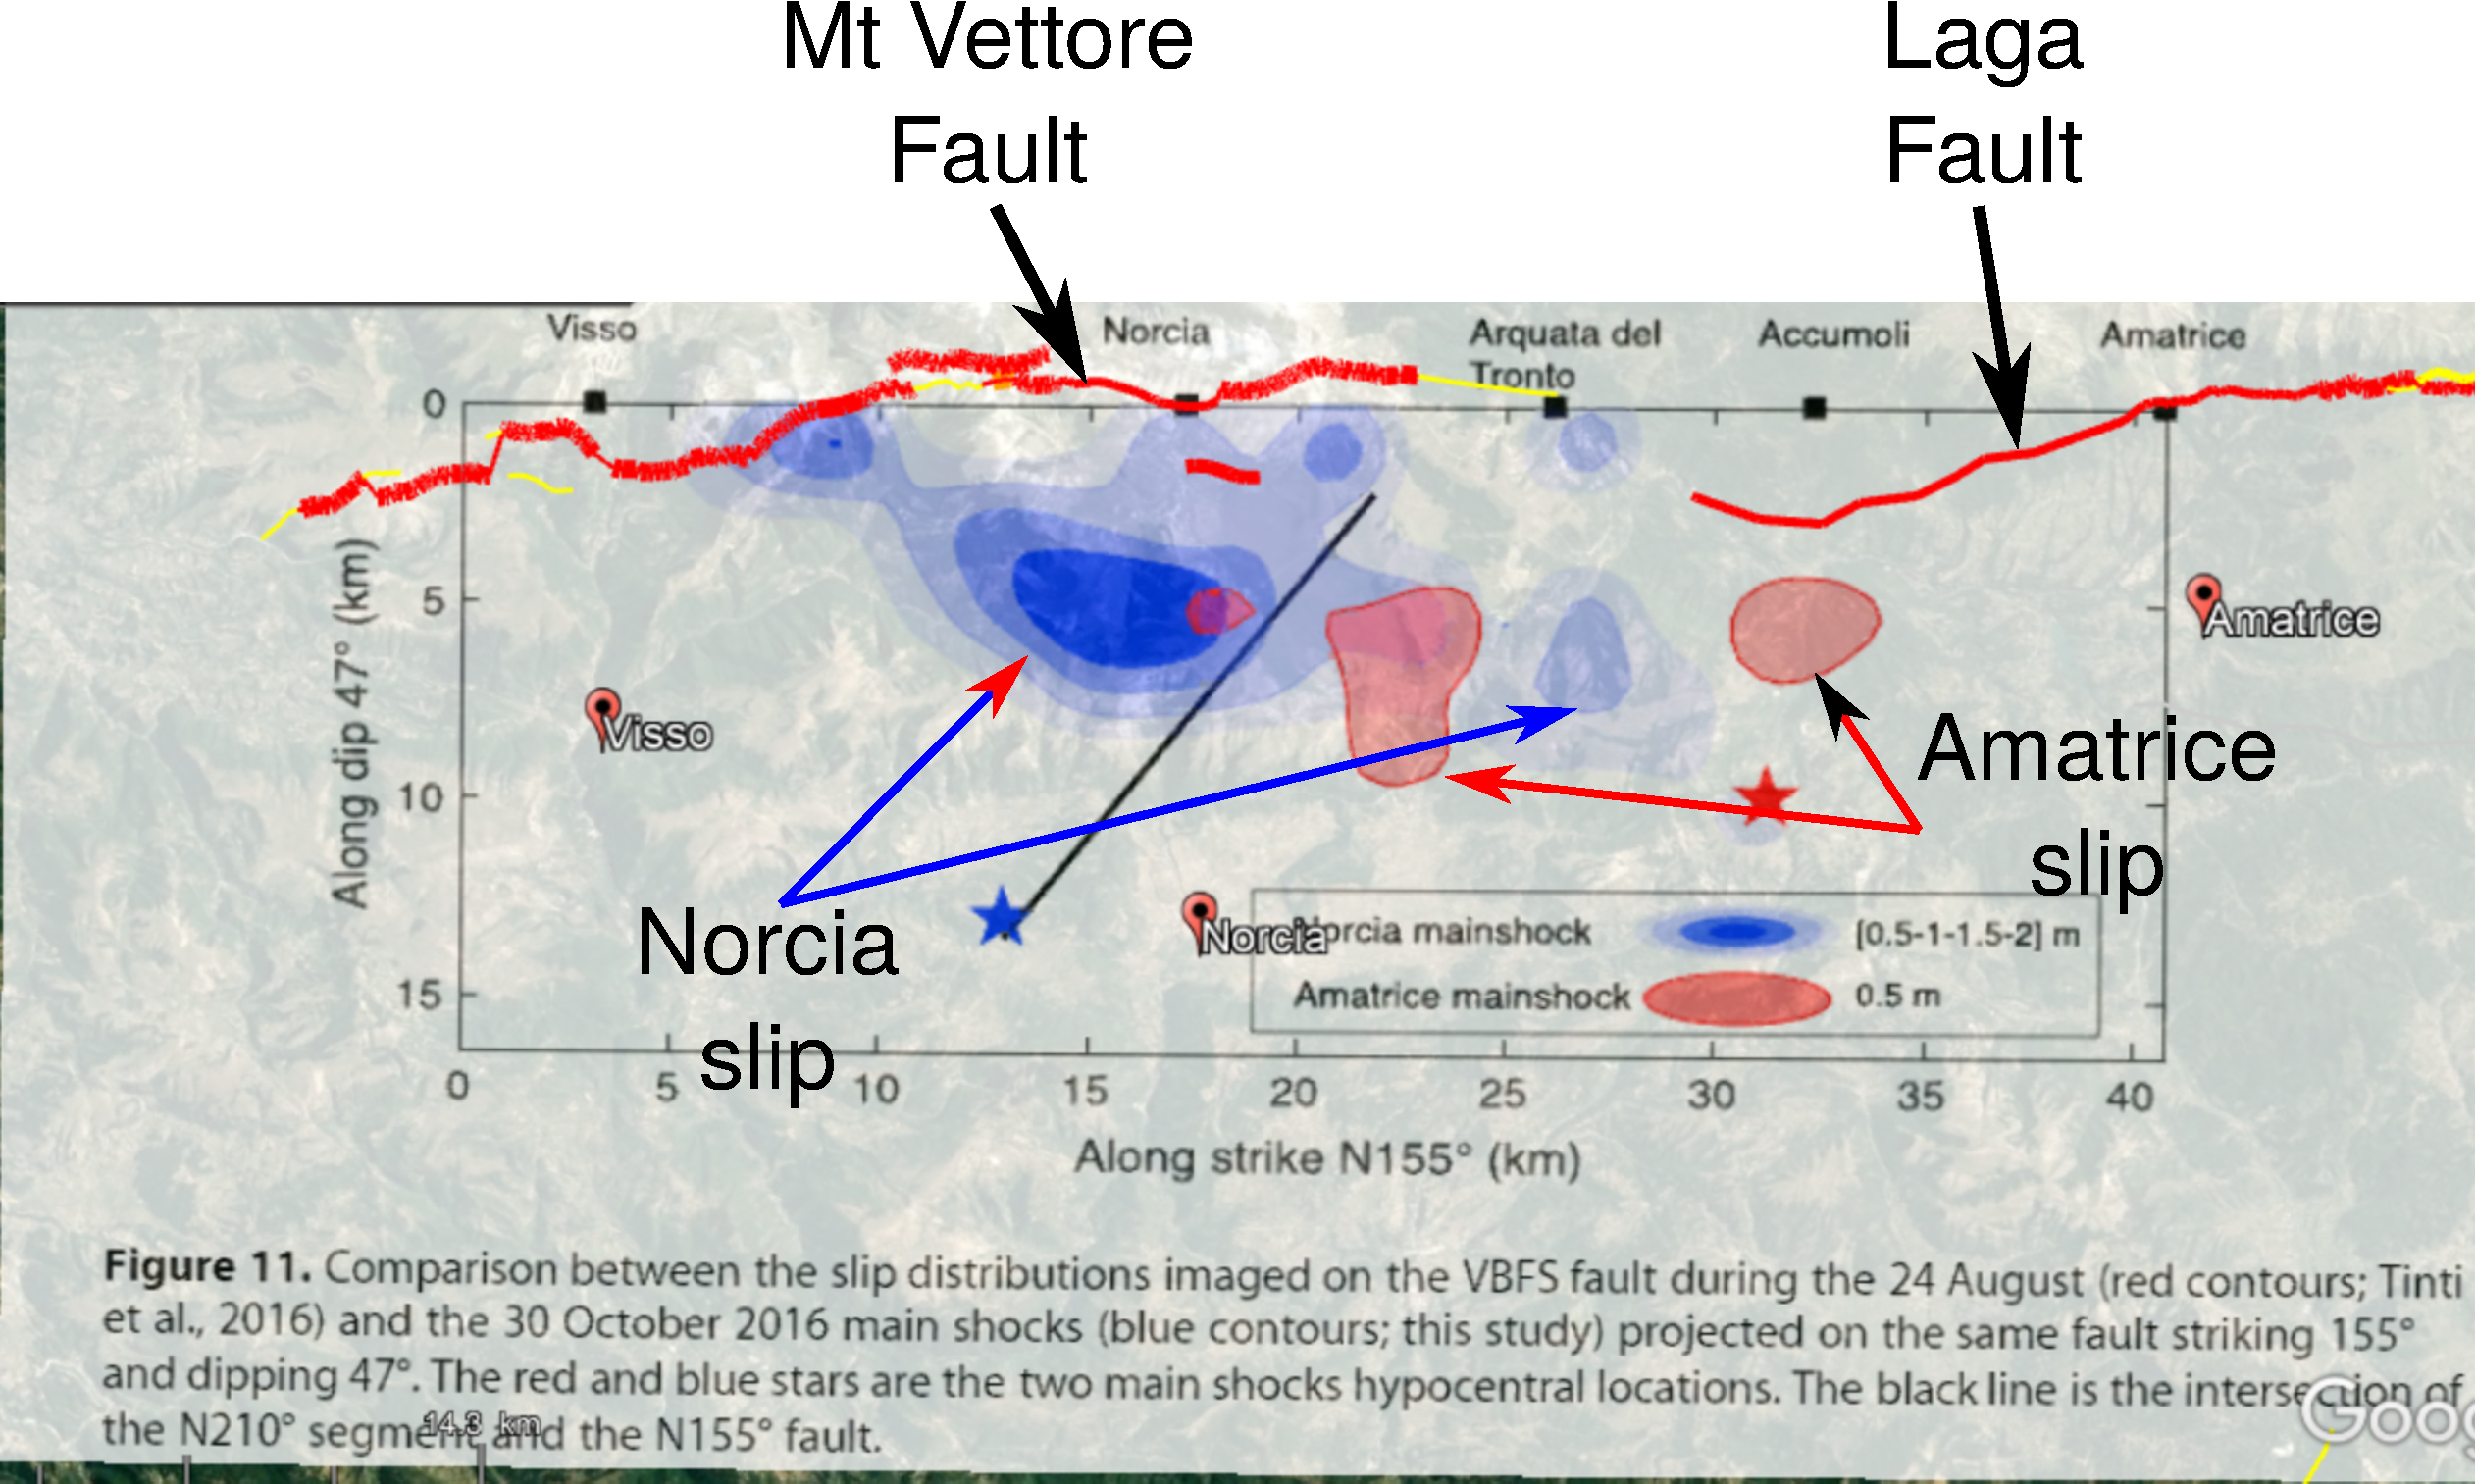
\includegraphics[width=1\linewidth]{images/amatrice_3.pdf} \,
  \vskip 0.2cm
  {\bf \tiny Modified by O. Scotti from \cite{Scognamiglio_2018_CFG}} \end{minipage}
 \begin{minipage}{0.33\linewidth}
  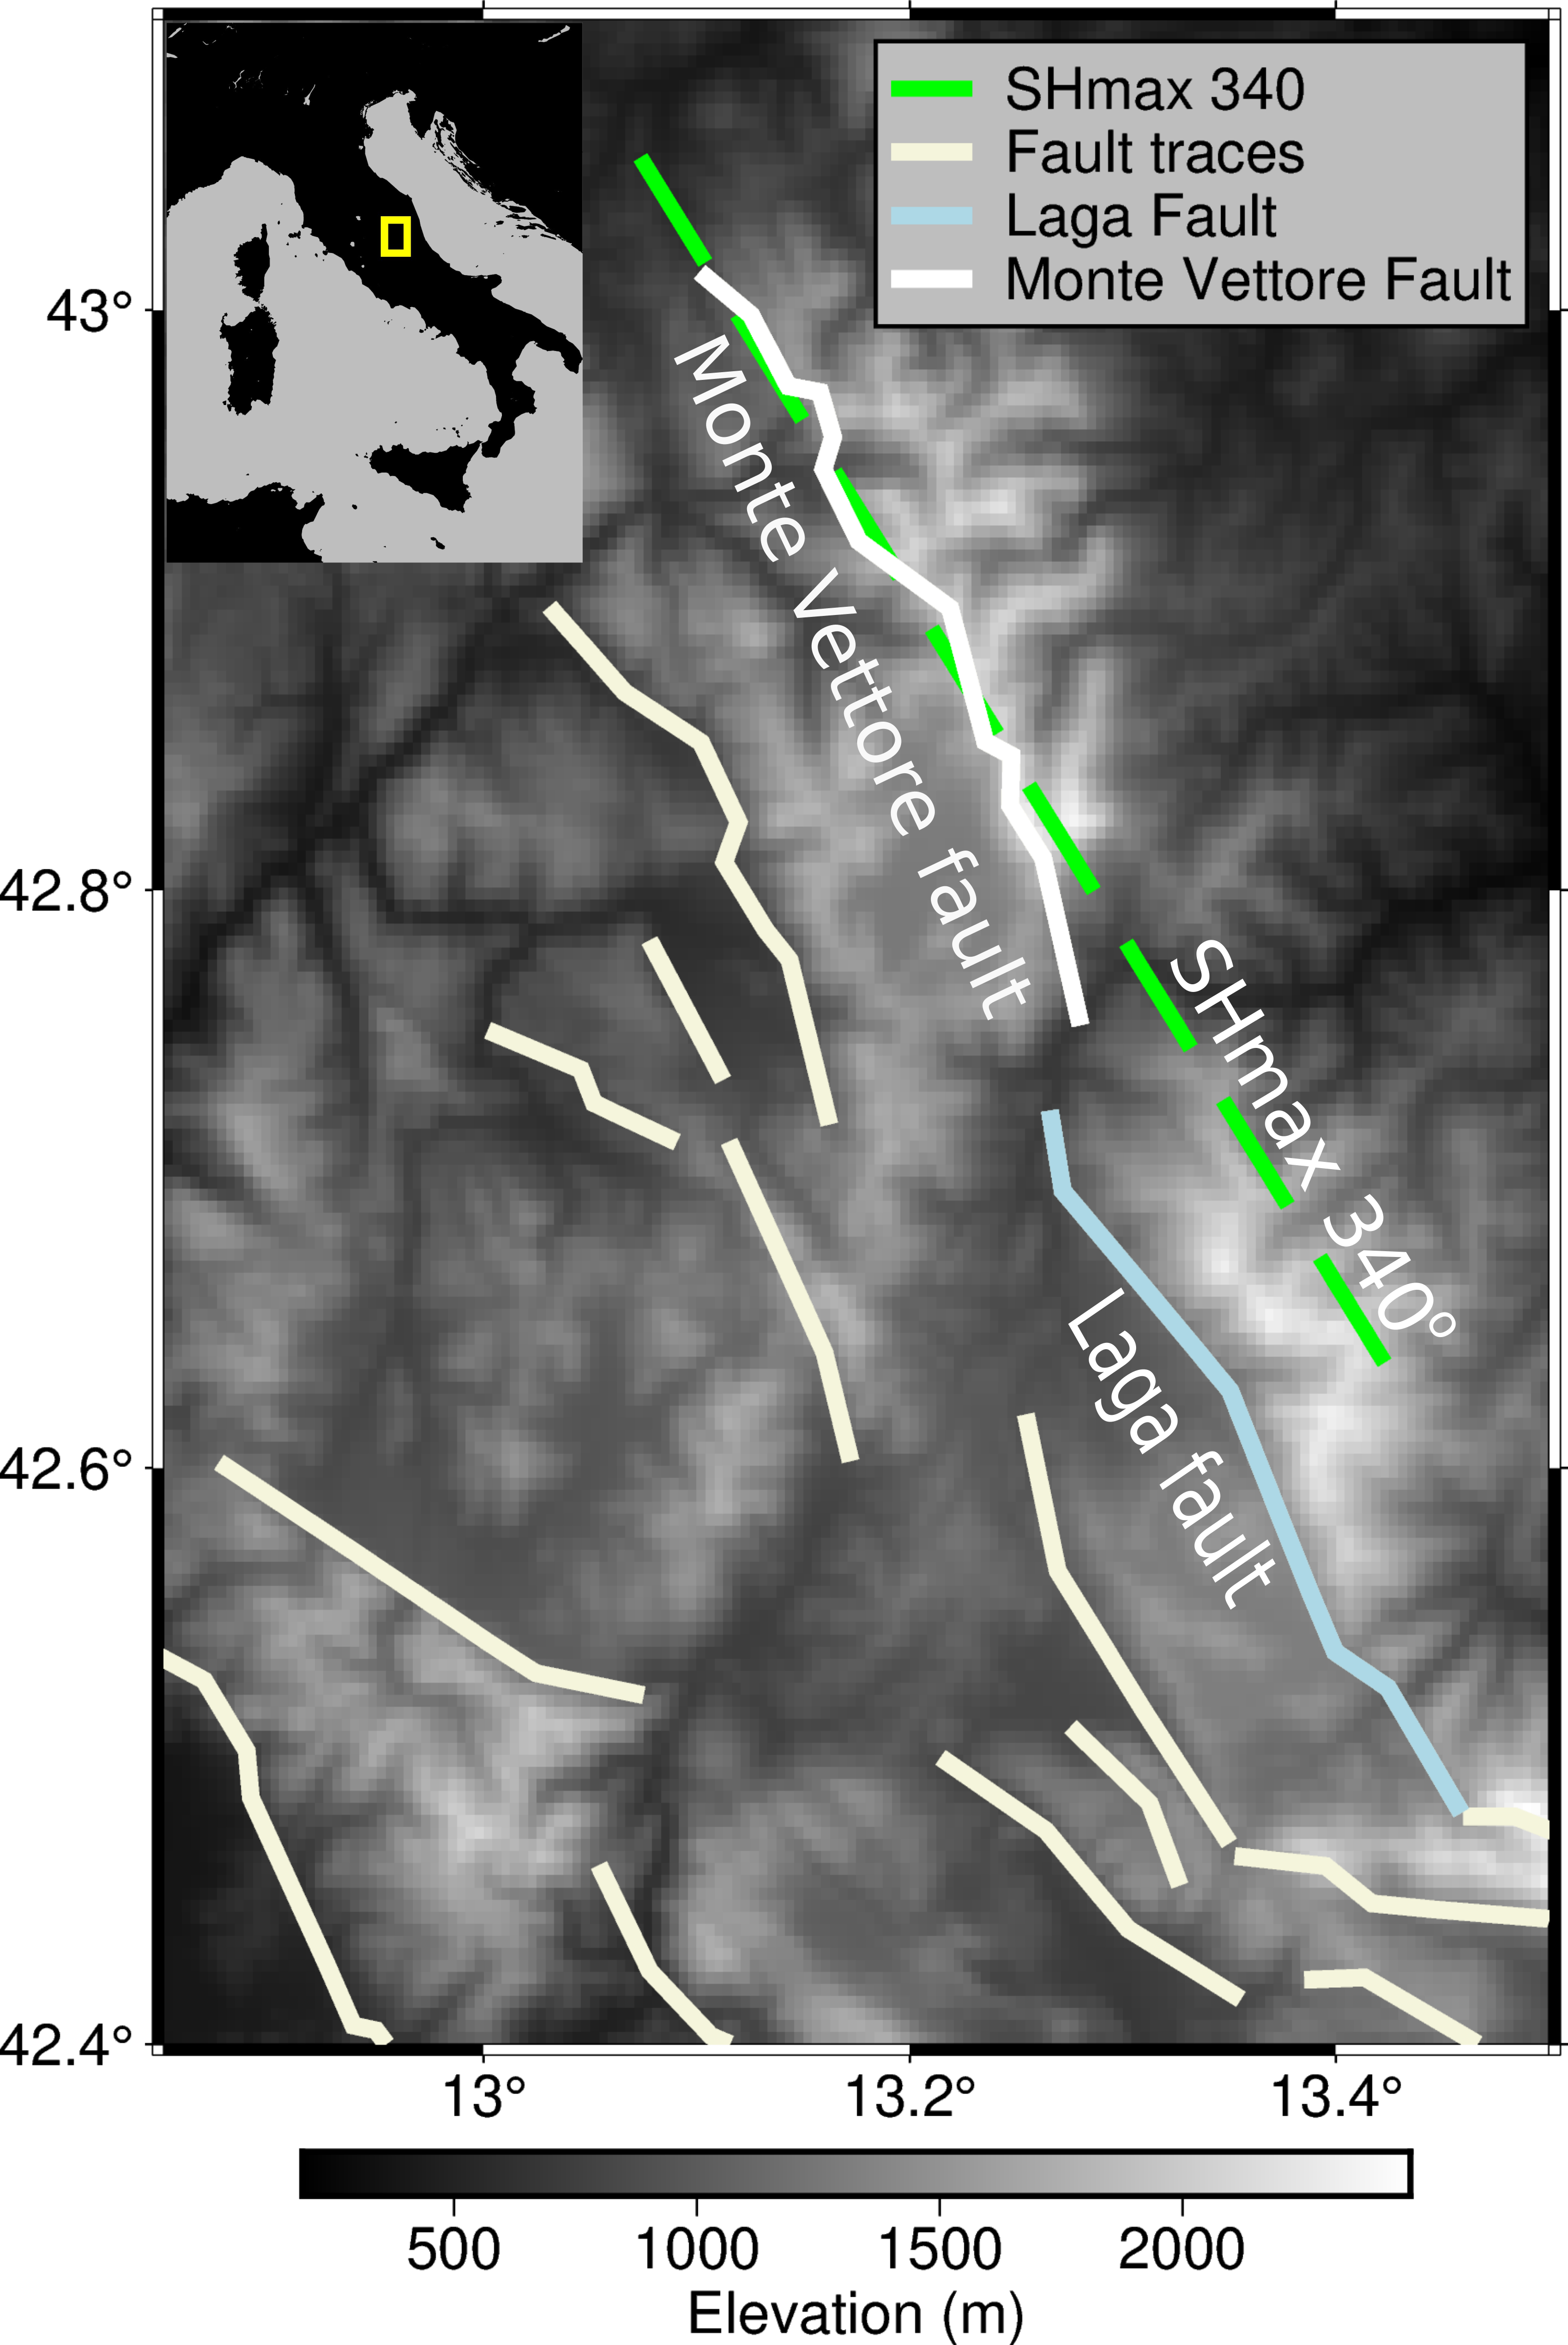
\includegraphics[width=1\linewidth]{images/Map_Italy.png}  
  \vskip 0.2cm
  {\bf \tiny Map based on \cite{Walker_2021_FAULT2SHA}} \end{minipage}
 \end{center}
 \end{center}
  \addtocounter{framenumber}{-1}
  
\end{frame}


\begin{frame}
 {Seismic Hazard in Central Italy}
 
 \begin{center}
  \begin{center}
 \begin{minipage}{0.65\linewidth}
  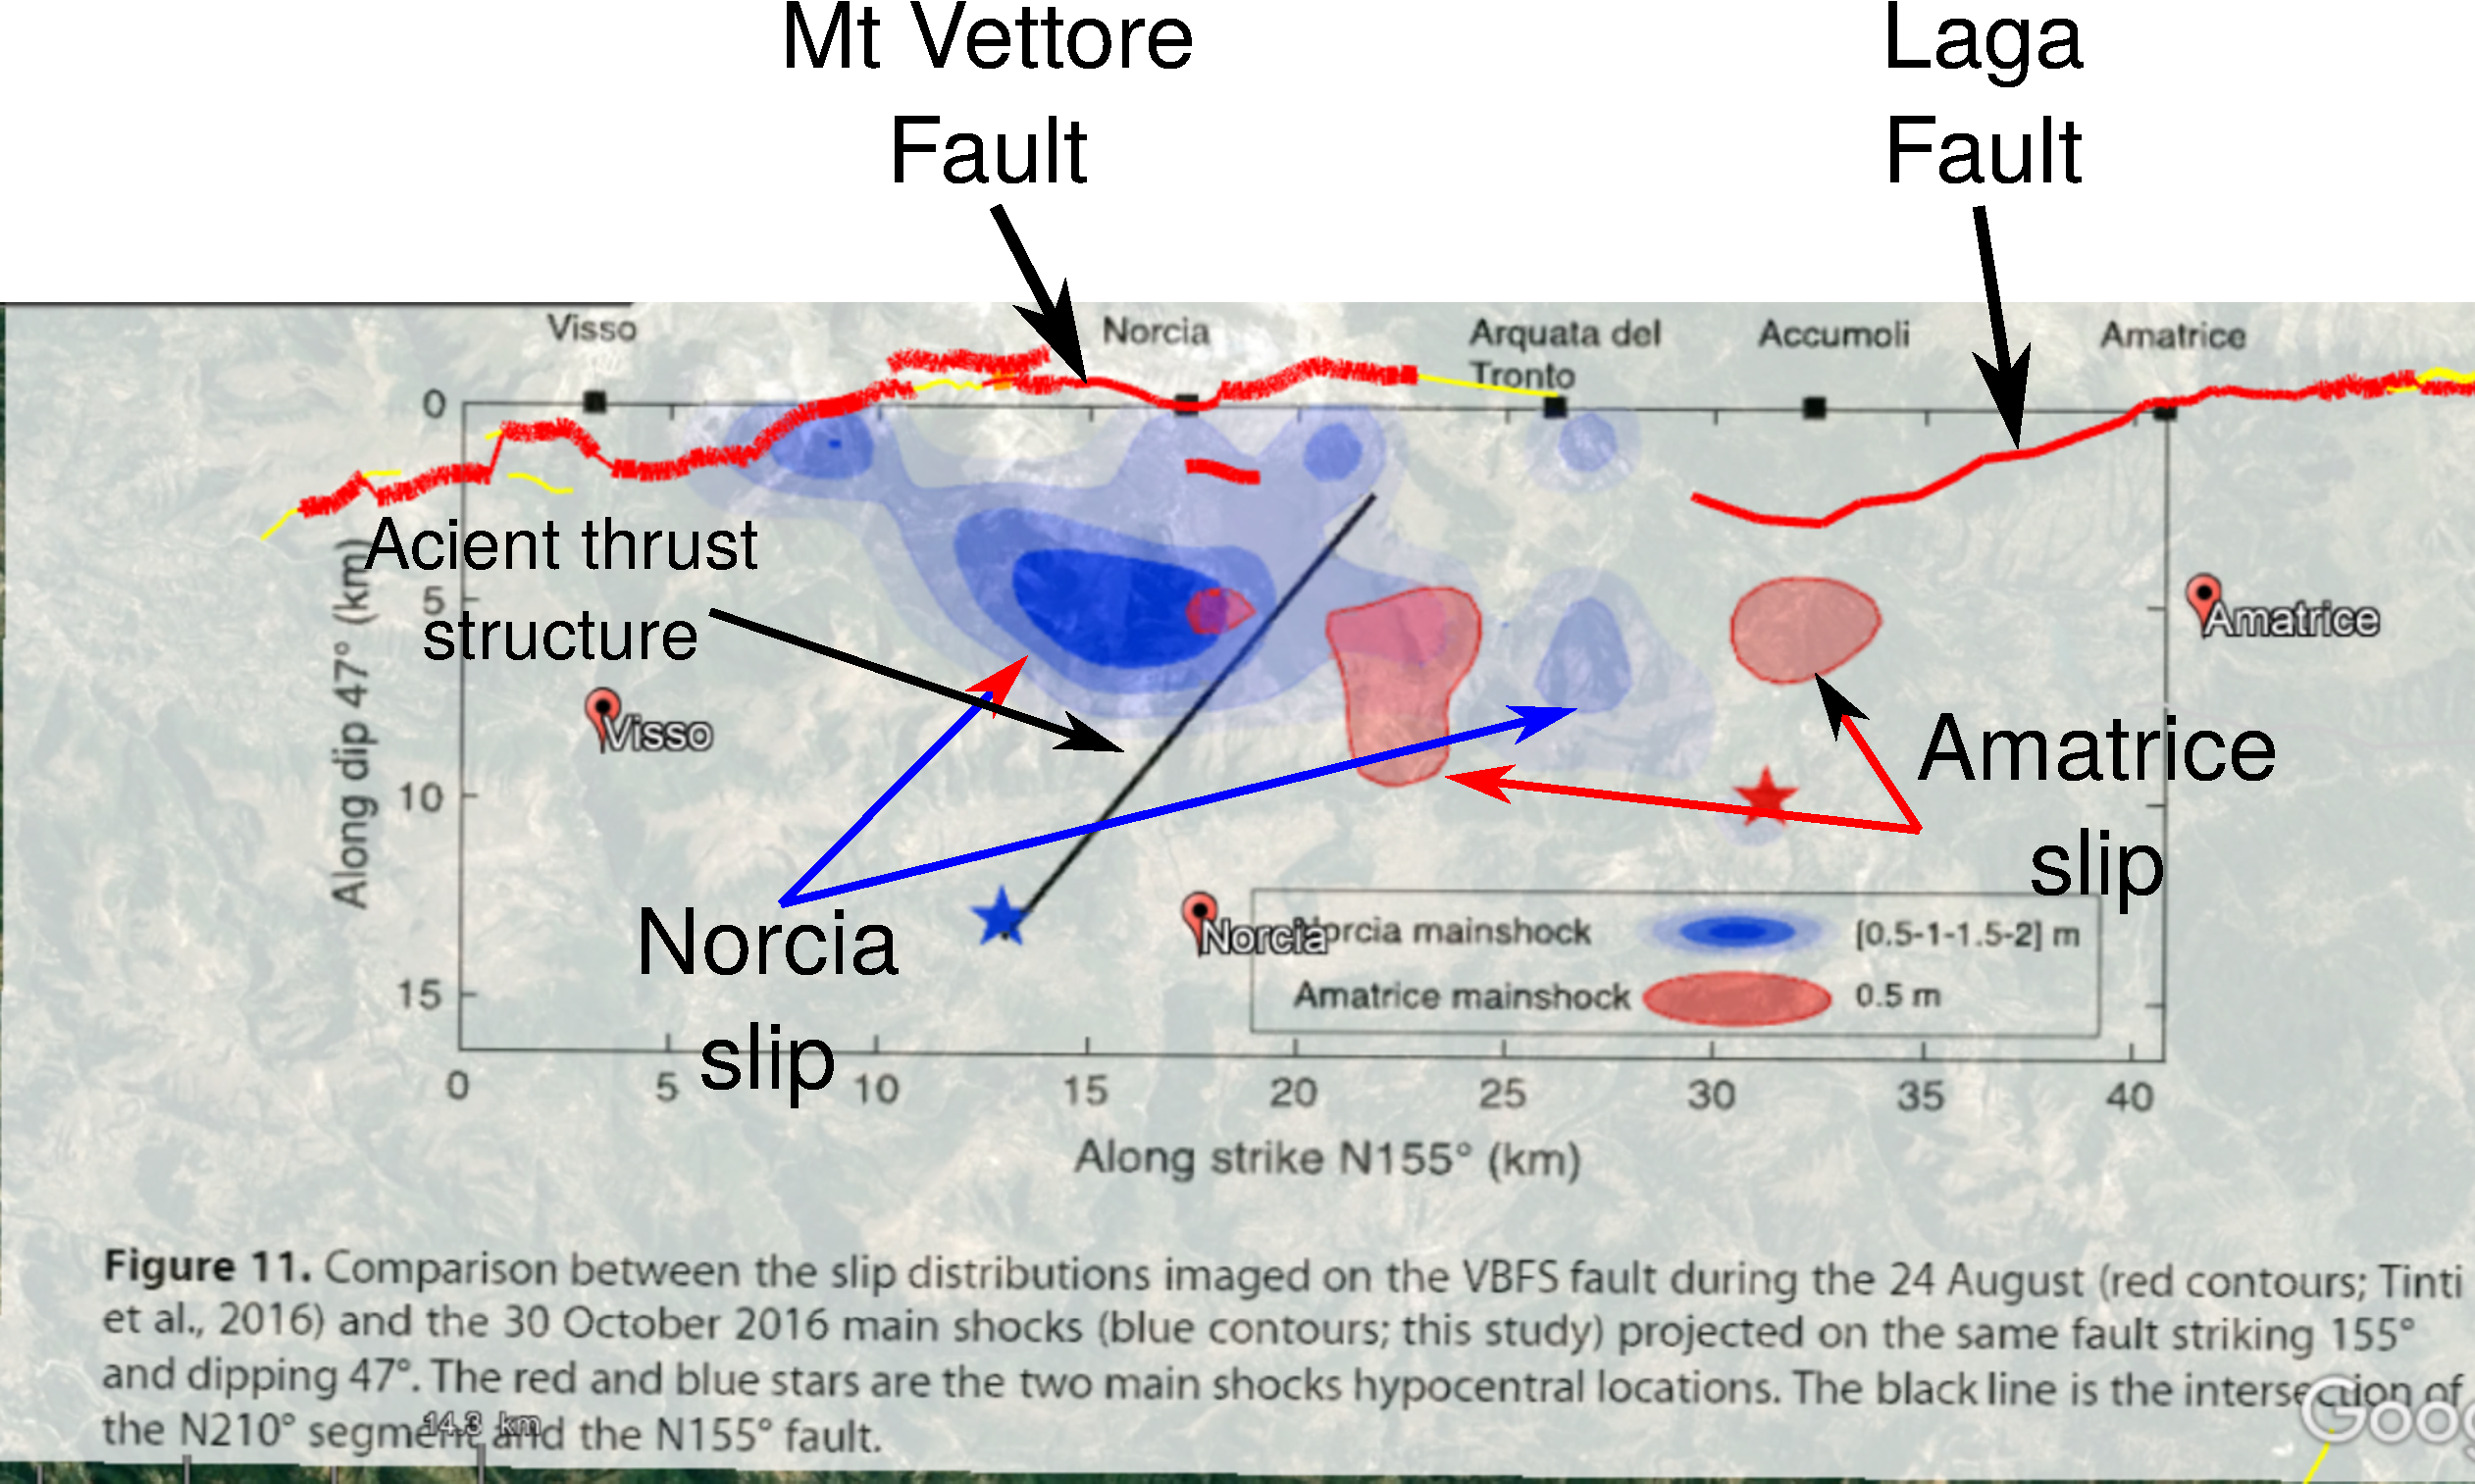
\includegraphics[width=1\linewidth]{images/amatrice_4.pdf} \,
  \vskip 0.2cm
  {\bf \tiny Modified by O. Scotti from \cite{Scognamiglio_2018_CFG}} \end{minipage}
 \begin{minipage}{0.33\linewidth}
  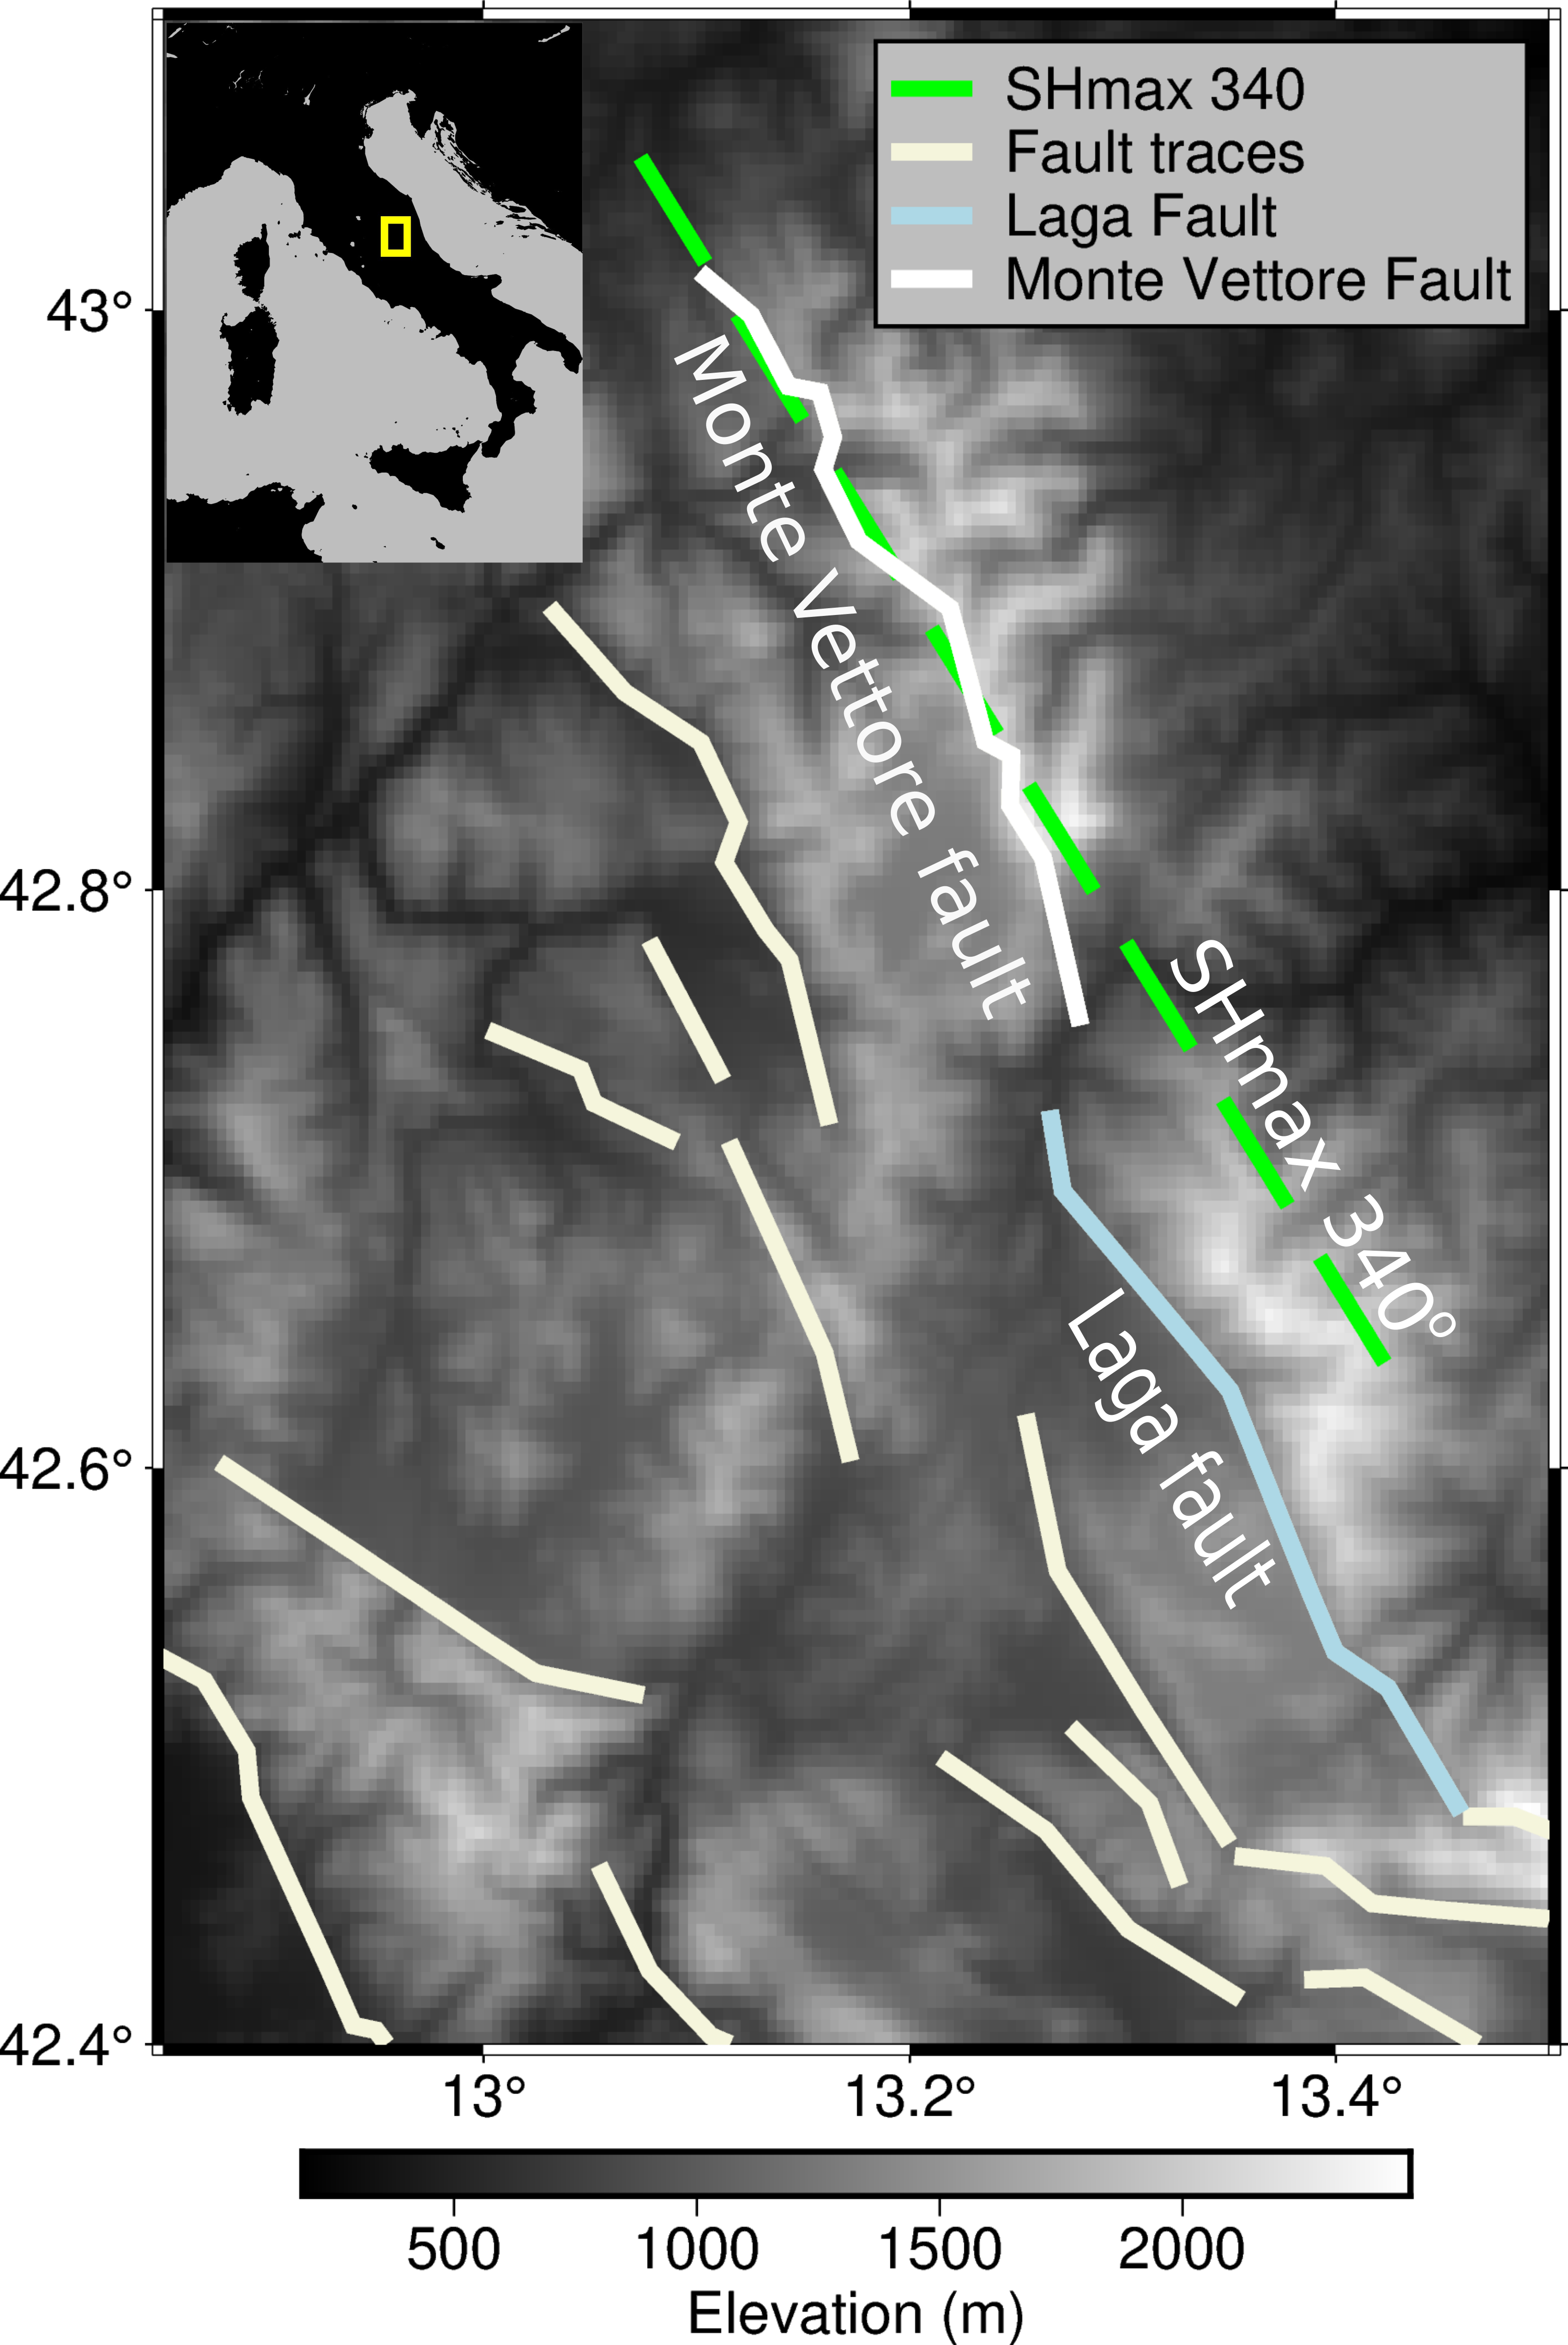
\includegraphics[width=1\linewidth]{images/Map_Italy.png}  
  \vskip 0.2cm
  {\bf \tiny Map based on \cite{Walker_2021_FAULT2SHA}} \end{minipage}
 \end{center}
 \end{center}
  \addtocounter{framenumber}{-1}
  
\end{frame}


\begin{frame}
 {Rupture jumps across step-overs}

  {\scriptsize \textbf{Previous studies focused on strike-slip fault systems:} \cite{Galis_2015_ISS,Hu_2016_IEJ,Bai_2017_ESD,Li_2020_ERT,Oglesby_2008_RTJ}, and more ... } \pause
 \vskip 0.2cm
 \begin{minipage}{0.45\linewidth}
  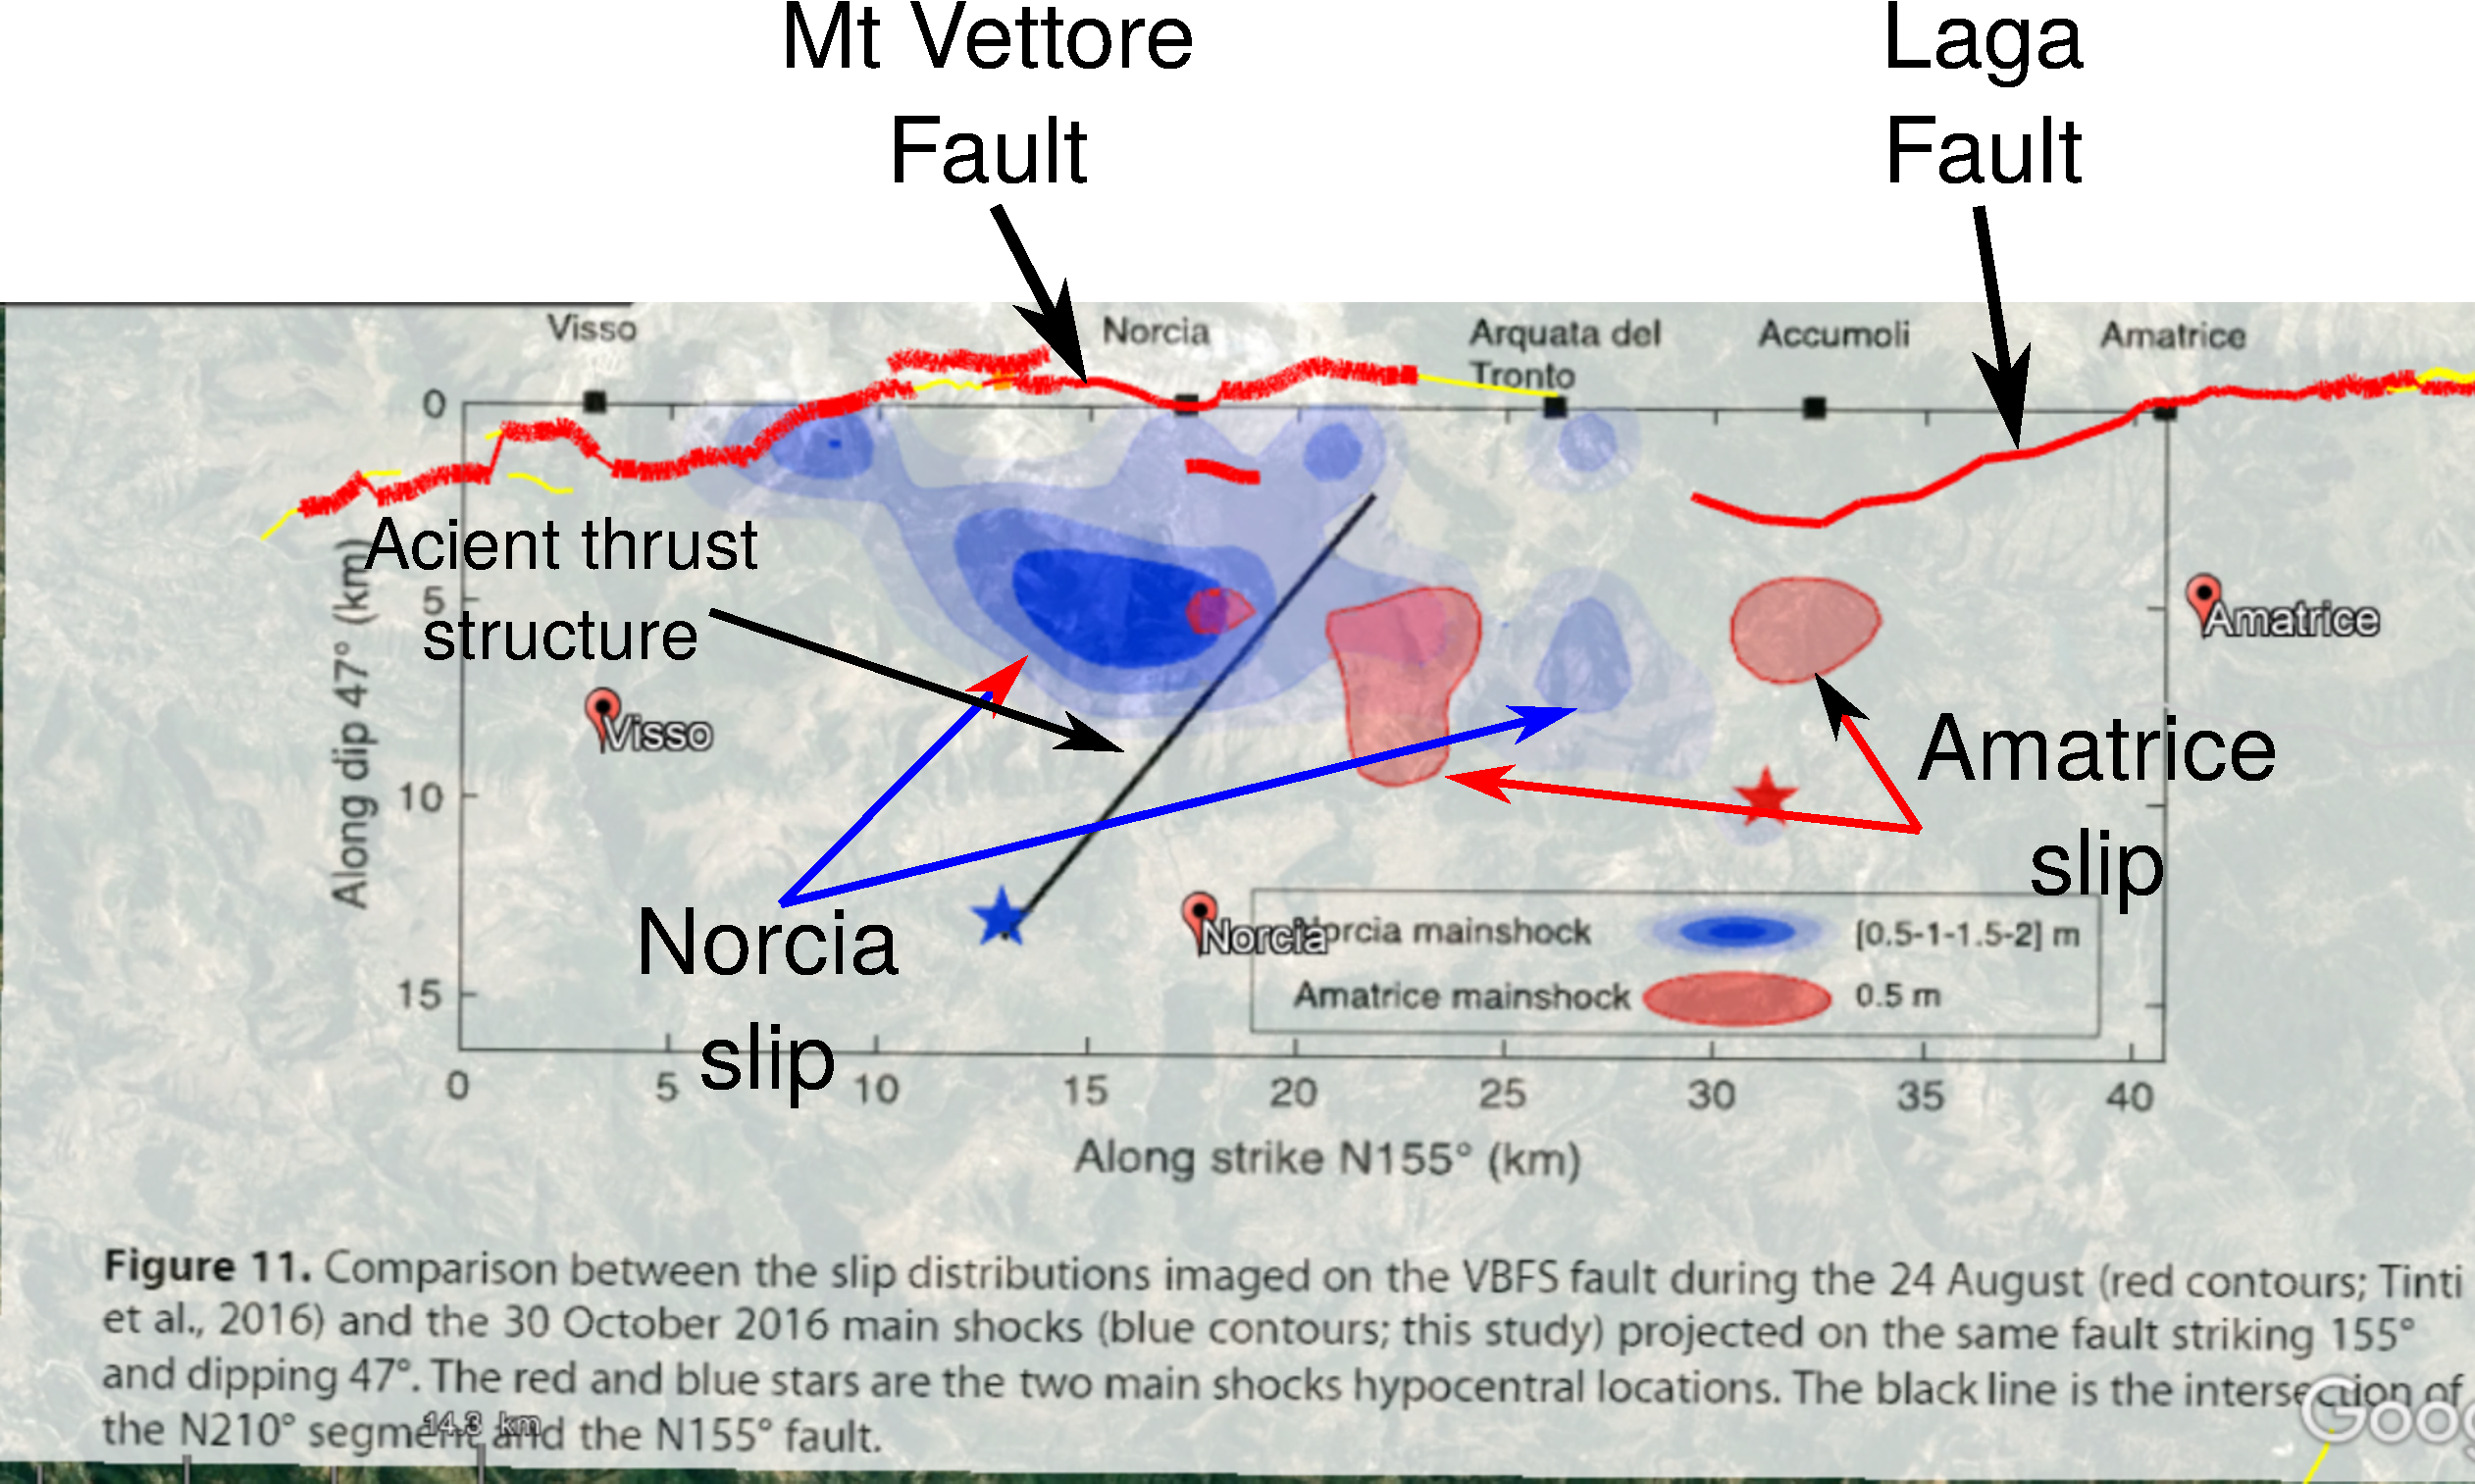
\includegraphics[width=1\linewidth]{images/amatrice_4.pdf}
 \end{minipage}
 \begin{minipage}{0.52\linewidth}
  {\bf \footnotesize In Central Italy:}
  \begin{itemize}
   \footnotesize \item \footnotesize Complex normal faulting systems  \pause
   \footnotesize \item \footnotesize Potential larger magnitudes? \pause
   \item \footnotesize Conditions promoting this? \pause
   \begin{itemize}
   \vskip 0.3cm
    \item \footnotesize Geometry \pause
    \item \footnotesize Stress conditions \pause
   \end{itemize}
   \vskip 0.3cm
   \item \footnotesize To enhance SHA! \pause
  \end{itemize}
 \end{minipage}

 \begin{center}
 \vskip 0.3cm
   \underline{\bf \small Investigate the physical conditons}
   \underline{\bf \small promoting rupture jumps across step overs} 
   \underline{\bf \small regarding normal fault systems} 
  \vskip 0.3cm
  
 \end{center}
 %\addtocounter{framenumber}{-1}
 
\end{frame}




\section{Settings}

\begin{frame}
 {Geometry and parameters explored}

 \vskip -0.2cm
  \includegraphics[width=1\linewidth]{images/model_no_table}
 \begin{minipage}{0.45\linewidth}
   {\scriptsize www.seissol.org} \\ {\tiny \citep[e.g.,][]{Wollherr_2018_OFP, Ulrich_2019_CPB}}
 \end{minipage}
 \begin{minipage}{0.45\linewidth}
 \hskip 2cm \vskip -0.7cm \begin{tabular}{l | r | r | r}
  Parameter           & $\min$ & $\Delta$ & $\max$  \\ \pause
  Offset (km)         & -5     & 2.5      & +5      \\ \pause
  Gap (km)            & -5     & 1        & +5      \\ \pause
  $S$                 & 0.1    & 0.1      & 0.3     \\ \pause
  SH$_{\max}$ ($^o$)  & 330    & 10       & 350     \\ \pause
 \end{tabular}
 \end{minipage}

\end{frame}


\begin{frame}
 {Static analysis ... jump? break-away?}
 
 \begin{center}
 \begin{minipage}{0.7\linewidth}
  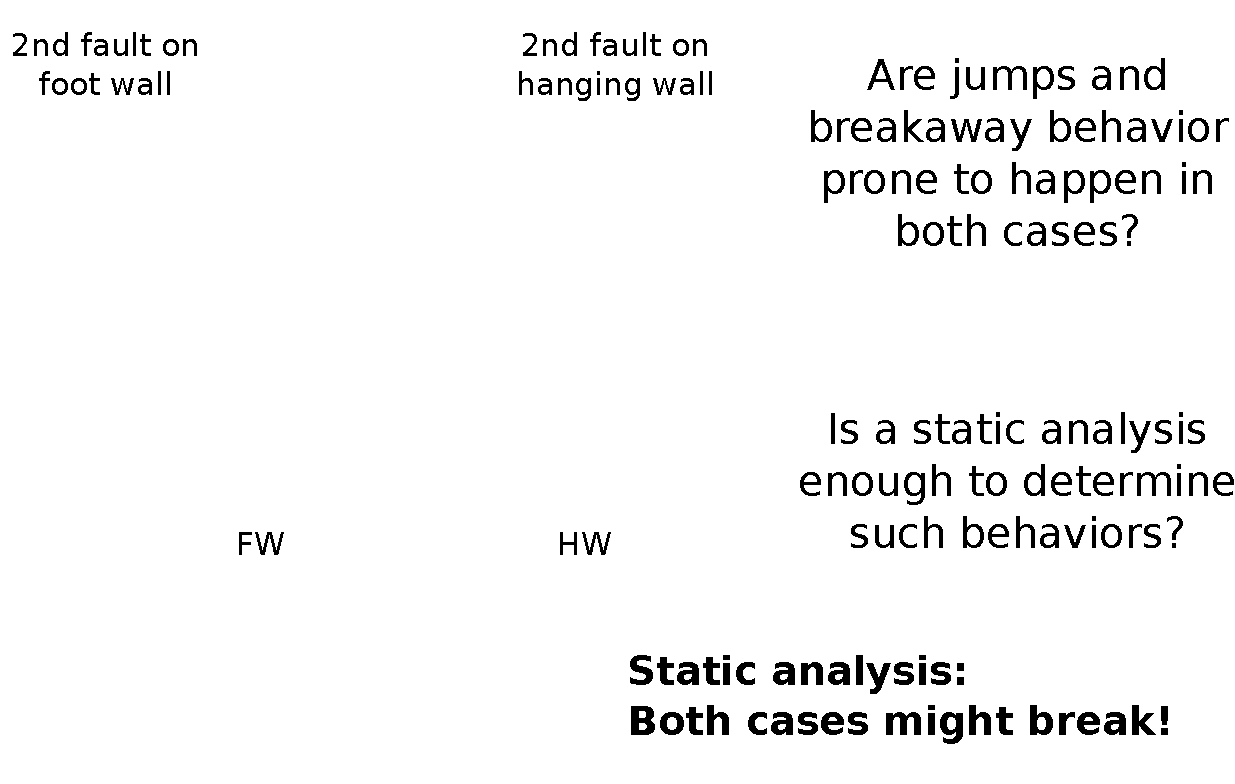
\includegraphics[width=1\linewidth]{images/static_analysis}
 \end{minipage}
 \end{center}

 
\end{frame}



\section*{References}
\begin{frame}

    {\tiny \bibliography{\dirbiblio/bibliography} }							\bibliographystyle{apalike}    

\end{frame}


\end{document}

